\appendix
\onecolumn
\section{Proof of Competitive Ratio for \algoname Algorithm}
\label{appendix:virtual_plus_proof_k_2}

As an illustrative example that aids in understanding the full general-$k$ proof for for the competitive ratio \algoname\ we now prove Theorem \ref{thm:general_k_theorem1} for $k=2$ from the main paper. 

\begin{theorem}  For $k=2$, the competitive ratio achieved by \algoname\ algorithm is equal to, 
\begin{equation}
    C_n = \frac{t(t-1)}{n} \sum_{j=t}^{n-1}\frac{1}{j(j-1)} \left(1 + 2 \sum_{ p=t+1}^j \frac{1}{p-1}\right)
\end{equation}
Particularly for $t= \alpha \cdot n\,,\, \alpha \in (0,1)$ we get 
\begin{equation} \label{eq:lower_bound_alpha1}
    C_n > \alpha ( 3(1-\alpha) + 2 \alpha \ln(\alpha)) + \mathcal{O}(1/n)
\end{equation}
Thus, asymptotically  we have
\begin{equation}
    C >  \max_{\alpha \in [0,1]} \alpha ( 3(1-\alpha) + 2 \alpha \ln(\alpha)) > .4273 > 1/e \, .
\end{equation}
\end{theorem}

\begin{figure}[ht]
    \centering
    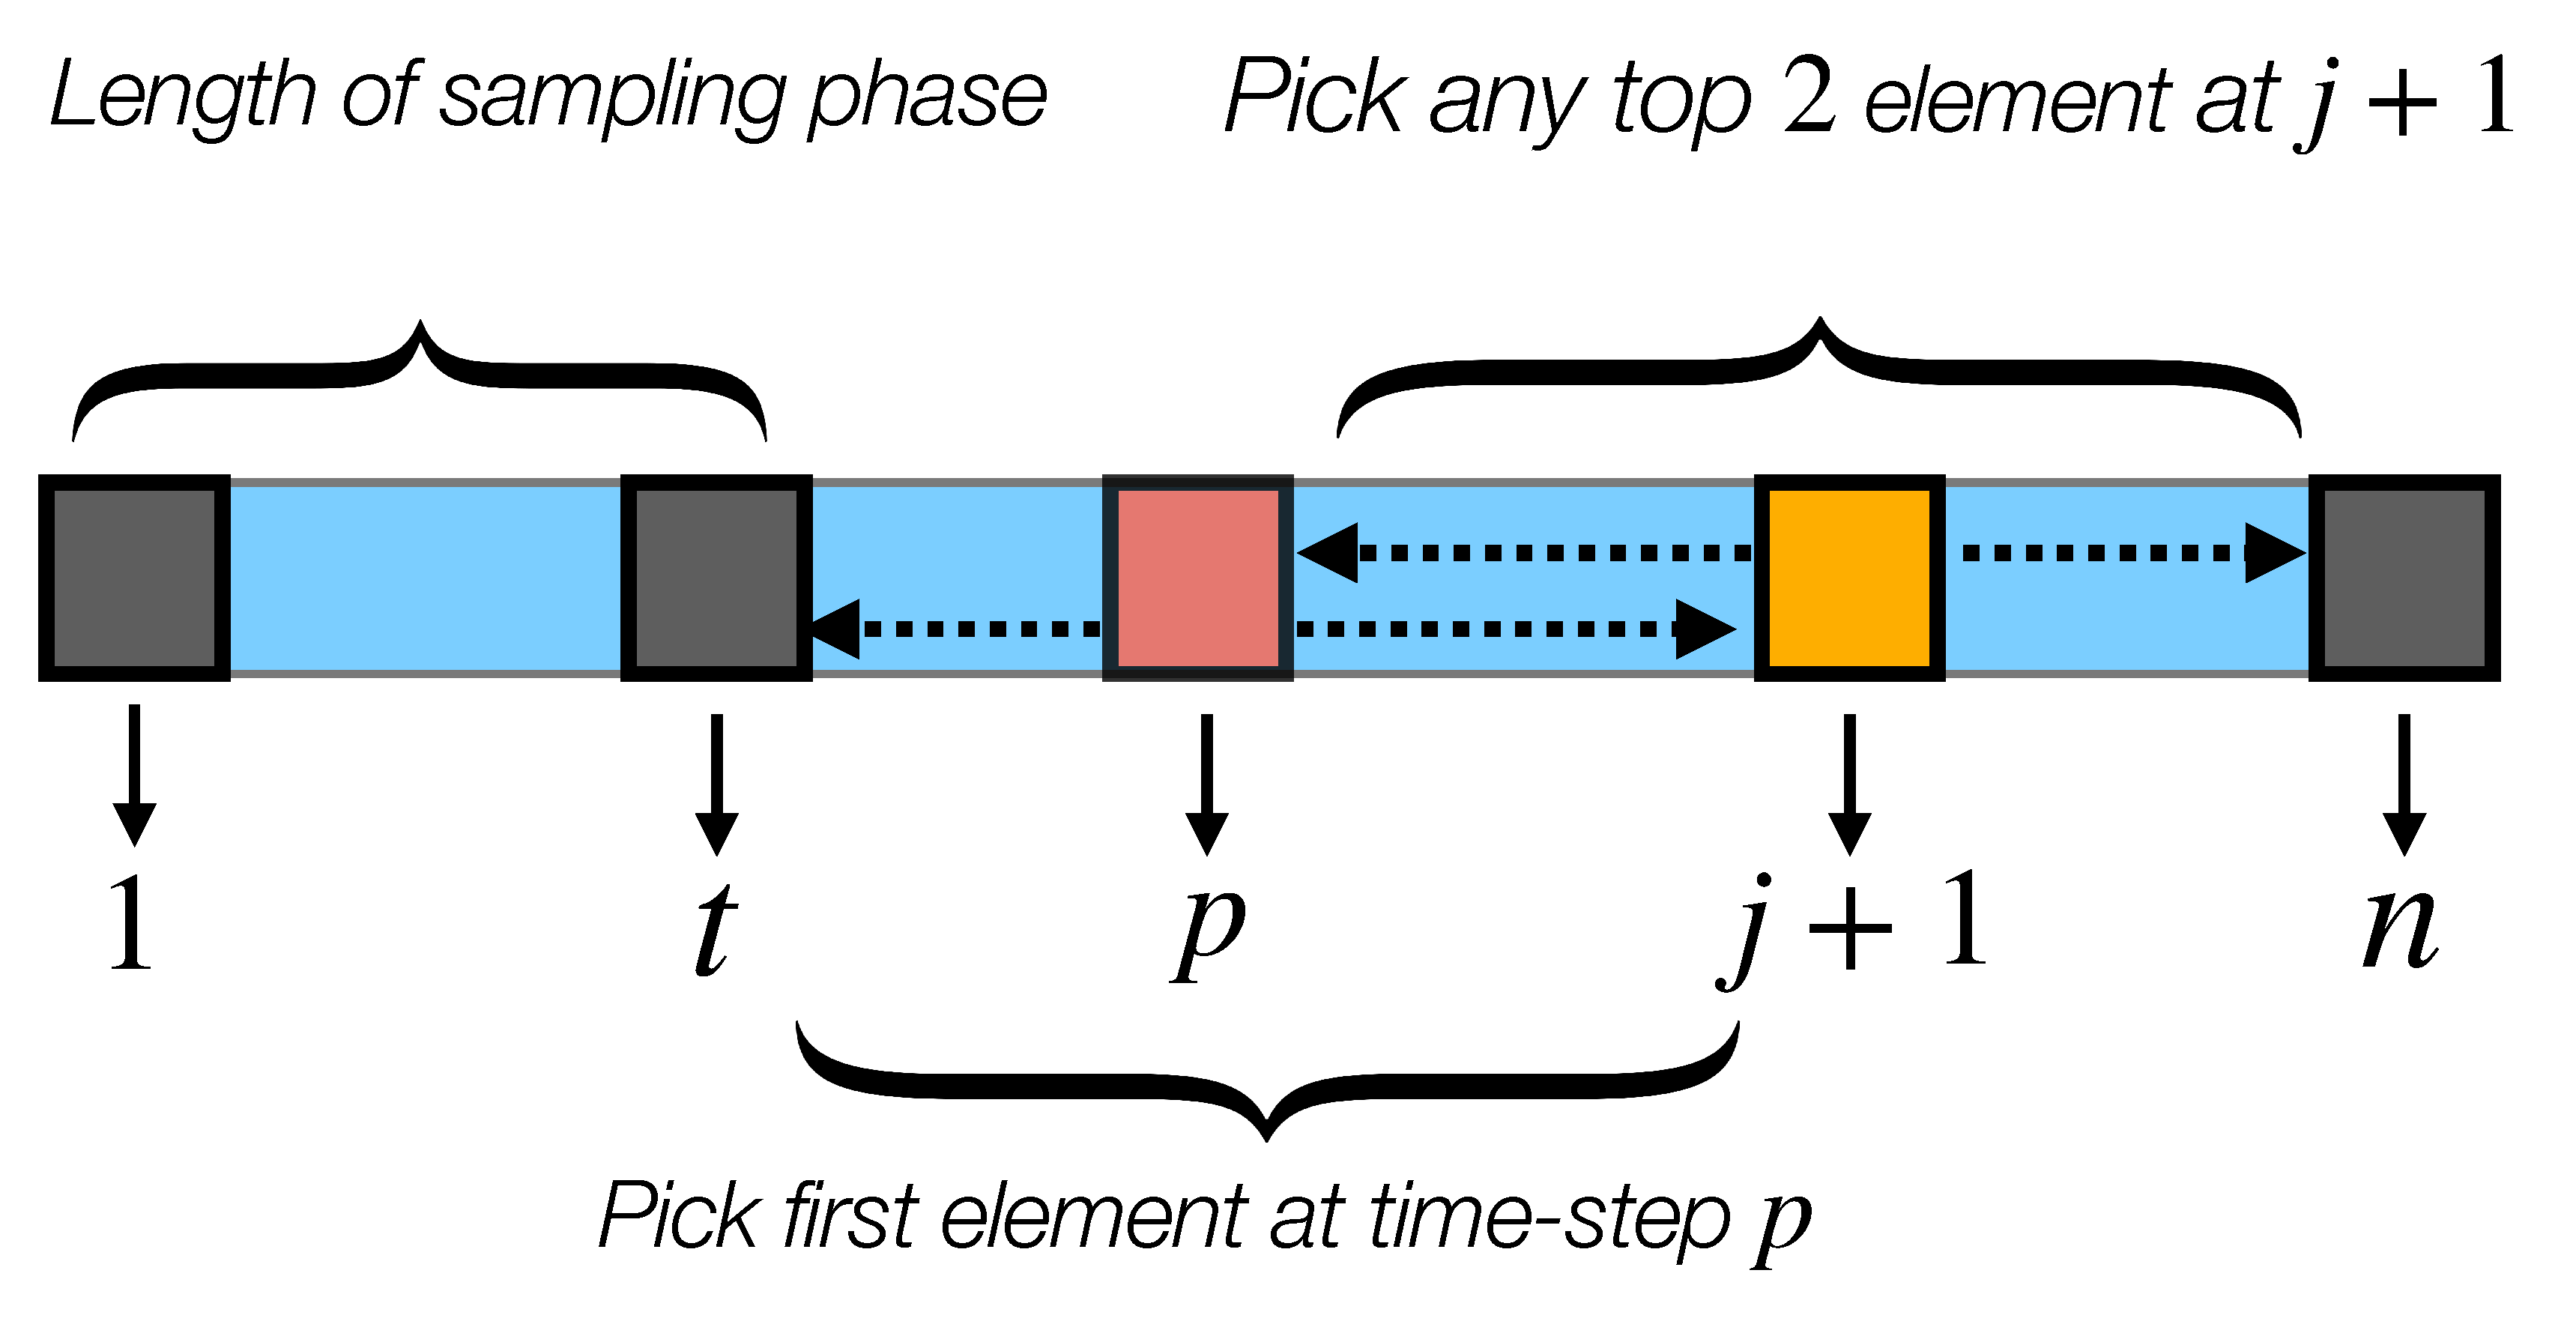
\includegraphics[width=1.0\linewidth]{Figures/virtual_plus_k_2.pdf}
    %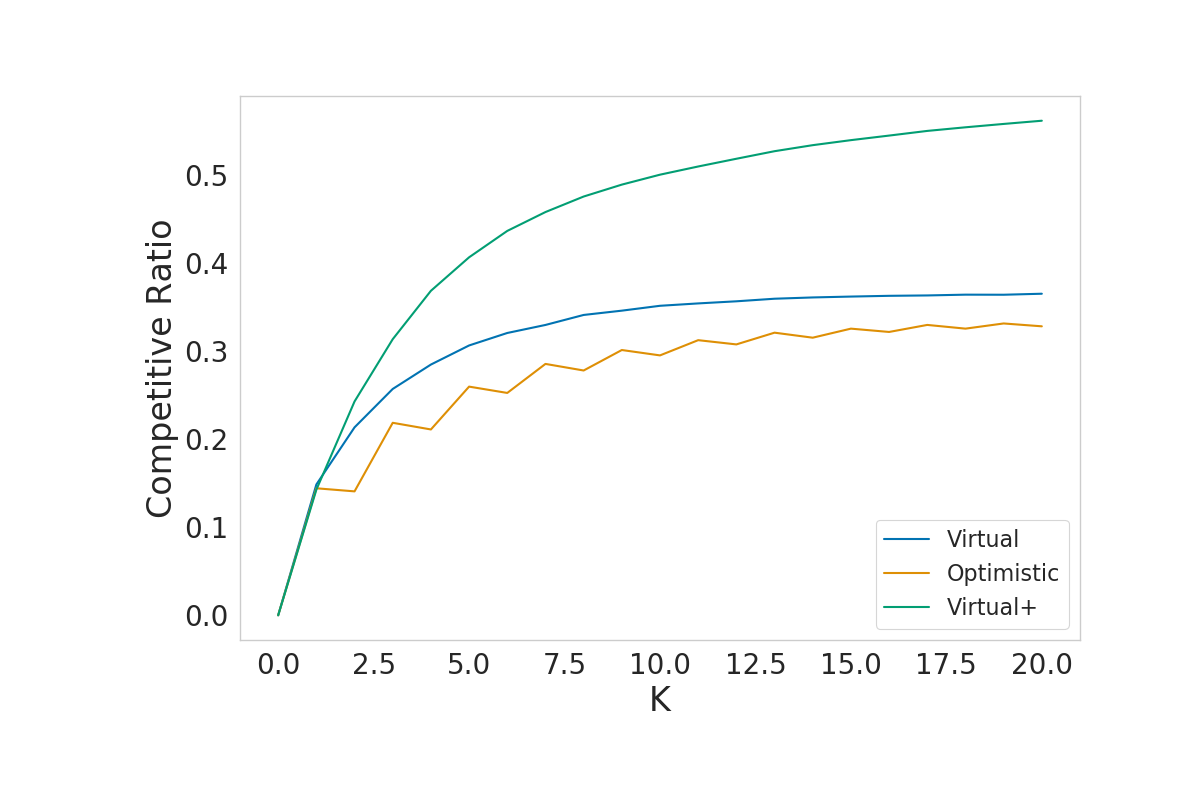
\includegraphics[width=\linewidth]{Figures/Competitive_RatioVar5.png}
    \caption{Probability of having only one element in $S_{\mathcal{A}}$ after $j$ time-steps with the \algoname\ algorithm.}
    \label{fig:k_2}
    \vspace{-15pt}
\end{figure}

\begin{proof}
First note that by \citet[Lemma 3.3]{albers2020new} we can show that the competitive ratio for the $k$-secretary problem for a monotone algorithm is equal to 
\begin{equation}
\label{eq:C_as_sum_k_two}
    C = \frac{1}{k}\sum_{a=1}^k \mathbb{P}(i_a \in S_\mathcal{A}), %\label{eq:C_as_sum_prob1}
\end{equation}
where $i_a$ is the index of the $a^{th}$ secretary picked by the offline solution ---i.e. $i_a$ is a top-$k$ secretary of $\mathcal{D}$. By Lemma \ref{lemma_monotone} \algoname \ is a monotone algorithm and we may use ~\eqref{eq:C_as_sum_k_two}.
Now, let us focus on the case $k=2$.
When calculating the probability of either of the top two items in $\mathcal{D}$ being picked by the \algoname\ we must first compute the probability of one of the top-2 items being picked during the selection phase (time step $t+1 \dots n$). Now notice that \algoname\ picks an item at time step $j+1$ if and only if this is a top-2 item with respect to all of $\mathcal{D}$ and $|S_{\mathcal{A}}| \leq 2$ at time-step $j+1$. Let top-$2_j$ denote the two largest elements observed by $\mathcal{A}$ up to and inclusive of time step $j$. Thus, for $a \in \{1,2\}$, we have
\begin{align}
    \mathbb{P}(i_a \in S_\mathcal{A}) 
    &= \sum_{j=t}^{n-1} \mathbb{P}(i_a \in S_\mathcal{A} \text{ at time-step }j+1)\\ %\label{p_picked_equal_not_filled} \\
    &= \frac{1}{n}\sum_{j=t}^{n-1} \mathbb{P}(|S_{\mathcal{A}}| < 2 \text{ at time-step } j + 1) \notag
\end{align}

Now, we compute $\mathbb{P}(|S_{\mathcal{A}}| \leq 2 \text{ at time-step } j+1)$ by decomposing this probability into the following two events: A.) $|S_{\mathcal{A}}| = 0$ where the selection set is empty and B.) the event $|S_{\mathcal{A}}| = 1$ where exactly one item has been picked. We now analyze each event in turn.

\xhdr{Event A} In order for the event $|S_{\mathcal{A}}|=0$ to occur it implies that the algorithm does not select any items in the first $j$ rounds. This means both two top-$2_j$ elements must have appeared in the sampling phase. Thus the probability for this event is exactly $\frac{t(t - 1)}{j (j - 1)}$. 

\xhdr{Event B}
The second event is when $|S_{\mathcal{A}}|=1$ ---i.e. the algorithm picks exactly one element in the first $j$ rounds. The computation of this event is illustrated in Figure~\ref{fig:k_2}. Let's say that an element is picked at time step $p$. Now to compute the probability of Event B occurring we first make the following two observations:

\begin{enumerate}[label={\bf Observation \arabic*:}, topsep=0pt, parsep=0pt, leftmargin=69pt, itemsep=2pt]
    \item  In order for exactly one element to be picked at the time step $p \leq j$, this element must be one of the top-$2_j$ elements. Furthermore, this implies the other of the top-$2_j$ element ---i.e. the one not picked at $p$ must have appeared in the sampling phase. Note that if both top-$2_j$ elements appear after the sampling phase, the condition would be satisfied twice and two elements would be selected instead of exactly one, and if they both appeared during the sampling phase we return to Event A. As a result, the probability for this condition is given by $\frac{t}{j (j - 1)}$.  
    \item By observation 1. we know that the online algorithm $\mathcal{A}$ picks one of the top-$2_j$ at time step $p$ and the fact that the event under consideration is $|S_{\mathcal{A}}|=1$ the reference list $R$ from time step $p$ to $j+1$ must contain both top-$2_j$ elements. However, for $\mathcal{A}$ to pick \emph{only} at $p$ we also need to ensure that no elements are picked prior t to $p$. Therefore, before time step $p$ the reference list must contain  top-$2_{p}$ . Again by observation 1, we know that $R$ already contains one of the top-$2_j$ elements therefore we know it contains one of the  top-$2_p$ elements. Thus the probability of ensuring that the second  top-$2_p$ elements is also within $R$ by time step $p$ is $\frac{(t - 1)}{(p - 2)}$. Finally, since there are two top elements and they may appear in any order we must count the probability of Event B occurring twice.

\end{enumerate}


Overall we get:
\begin{equation}
    \frac{t(t - 1)}{j (j - 1)} + 2 \sum_{p = t + 1}^{j}\frac{1}{j}\frac{t}{j - 1}\frac{t-1}{p-2}
\end{equation}
Total probability:
\begin{align*}
    \frac{1}{n} \sum_{j = t}^{n-1}\left(\frac{t(t - 1)}{j (j - 1)} + 2 \sum_{p = t + 1}^{j}\frac{1}{j}\frac{t}{j - 1}\frac{t-1}{p-2}\right) 
    &= 
   \frac{1}{n}\sum_{j = t}^{n-1}\left(1 + 2\sum_{p=t}^{j - 1} \frac{1}{p - 1} \right) \\
   &= 
   \frac{t(t - 1)}{n}\sum_{j=t}^{n-1}\left(\frac{1}{j(j-1)} + \frac{2}{j(j-1)}\sum_{p = t}^{j-1}\frac{1}{p-1}\right)\\
   & >
   \frac{t(t-1)}{n}\sum_{j = t}^{n - 1}\left(\frac{1}{j^2} + 2\frac{1}{j^2}\sum_{p = t + 1}^{j}\frac{1}{p-1}\right) \\
   & >
   \frac{t(t-1)}{n}\sum_{j = t}^{n - 1}\left(\frac{1}{j^2} + \frac{2}{j^2}\int_{p=t+1}^{j+1} \frac{1}{p-1}\, dp \right)\\
   & >
   \frac{t(t-1)}{n}\sum_{j = t}^{n-1}\left(\frac{1}{j^2} + \frac{2}{j^2}\ln\left(\frac{j}{t}\right)\right)
%   =\frac{t(t-1)}{n}(\sum_{j = t}^{a}(\frac{1}{j^2} + \frac{2}{j^2}\ln(\frac{j}{t})) + \sum_{j = a + 1}^{n - 1}(\frac{1}{j^2} + \frac{2}{j^2}\ln(\frac{j}{t})))\\
%   &\textgreater
%   \frac{t(t-1)}{n}(\int)
%   | \int_n^{n+1} f(t) dt - f(n)| \leq \int |f(t) - f(n)| dt \leq \int sup_{[n,t]}|f'(x)||t-n| dt
\end{align*}
Now we will use the following lemma
\begin{lemma}
For any differentiable function $f$ and any $a<b$, we have,
\begin{equation}
    \sum_{j=a}^{b} f(j) \geq \int_a^{b+1} f(t) dt - |b+1-a|\sup_{t \in [a,b+1]} |f'(t)|
\end{equation}
\end{lemma}
\begin{proof}
\begin{equation}
     | f(n) - \int_n^{n+1} f(t) dt | \leq \int_n^{n+1} |f(n)-f(t)| dt \leq \sup_{t \in [n,n+1]} |f'(t)| 
\end{equation}
Thus, 
\begin{equation}
    f(n) \geq  \int_n^{n+1} f(t) dt - \sup_{t \in [n,n+1]} |f'(t)| 
\end{equation}
and by summing for $n = a \ldots b$ we get the desired lemma. 
\end{proof}
Applying this lemma to $f(x) = \frac{1+2\ln(x/t)}{x^2}\,, a = t$ and $b=n-1$, we get 
\begin{align}
    \frac{1}{n} \sum_{j = t}^{n-1}\frac{t(t - 1)}{j (j - 1)} + 2 \sum_{p = t + 1}^{j}\frac{1}{j}\frac{t}{j - 1}\frac{t-1}{p-2} 
    & > \frac{t(t-1)}{n}\sum_{j = t}^{n-1}\left(\frac{1}{j^2} + \frac{2}{j^2}\ln\left(\frac{j}{t}\right)\right) \\
    & \geq \frac{t(t-1)}{n}\left(\int_{t}^{n}  \frac{1+2\ln(x/t)}{x^2} dx - 2(n-t) \sup_{x \in [t,n]} \left| 
    \frac{4 \ln(x/t)}{x ^3}\right| \right) \notag \\
    & \geq  \frac{t(t-1)}{n}\left(\int_{t}^{n}  \frac{1+2\ln(x/t)}{x^2} dx - 2(n-t) \left| \frac{16}{3 t^3 e^4} \right| \right) \notag \\
    & = 
    \frac{t(t -1)}{n} \left(\frac{3}{t}-\frac{2\ln(n/t) + 3}{n} - 2(n-t) \left| \frac{16}{3 t^3 e^4} \right|\right) 
\end{align}
Now for $t = \alpha n$ where $\alpha \in (0, 1)$ and as $n \xrightarrow[]{} \infty$, that lower-bound becomes 
\begin{equation}
C \geq \alpha (3 - \alpha(3 - 2\ln (\alpha))) + \mathcal{O}(1/n) \,,\quad \forall \alpha \in (0,1)
\end{equation}
The constant term of the RHS is a concave function of $\alpha$ that is maximized for $\alpha^* \approx 0.38240$. Thus, our algorithms achieves competitive ratio larger than $0.42737$.
\end{proof}


\clearpage

\section{Competitive Ratio General $k$}
\label{app:general_k_proof}
We now prove our main result for the competitive ratio of \algoname \ for $k \geq 2$. The theorem statement is reproduced here for convenience.  
\begin{reptheorem}{thm:general_k_theorem1}
The competitive ratio of \algoname\ for $k \geq 2$ and where $t = \alpha n$ can asymptotically be lower bounded by 
\begin{equation}
    C_k >  \max_{\alpha \in [0,1]}  {\alpha}^k \left(\sum_{m = 0}^{k - 1} a_m \ln^m (\alpha)\right) - \alpha a_0
    \hspace{0.15cm }where  \hspace{0.15cm }
    a_m = \left(\frac{\frac{k^k}{(k-1)^{k-m}} - k^m}{m!}\right)(-1)^{m+1}
    \, .
\end{equation}

\end{reptheorem}
\begin{figure}[ht]
    \centering
    %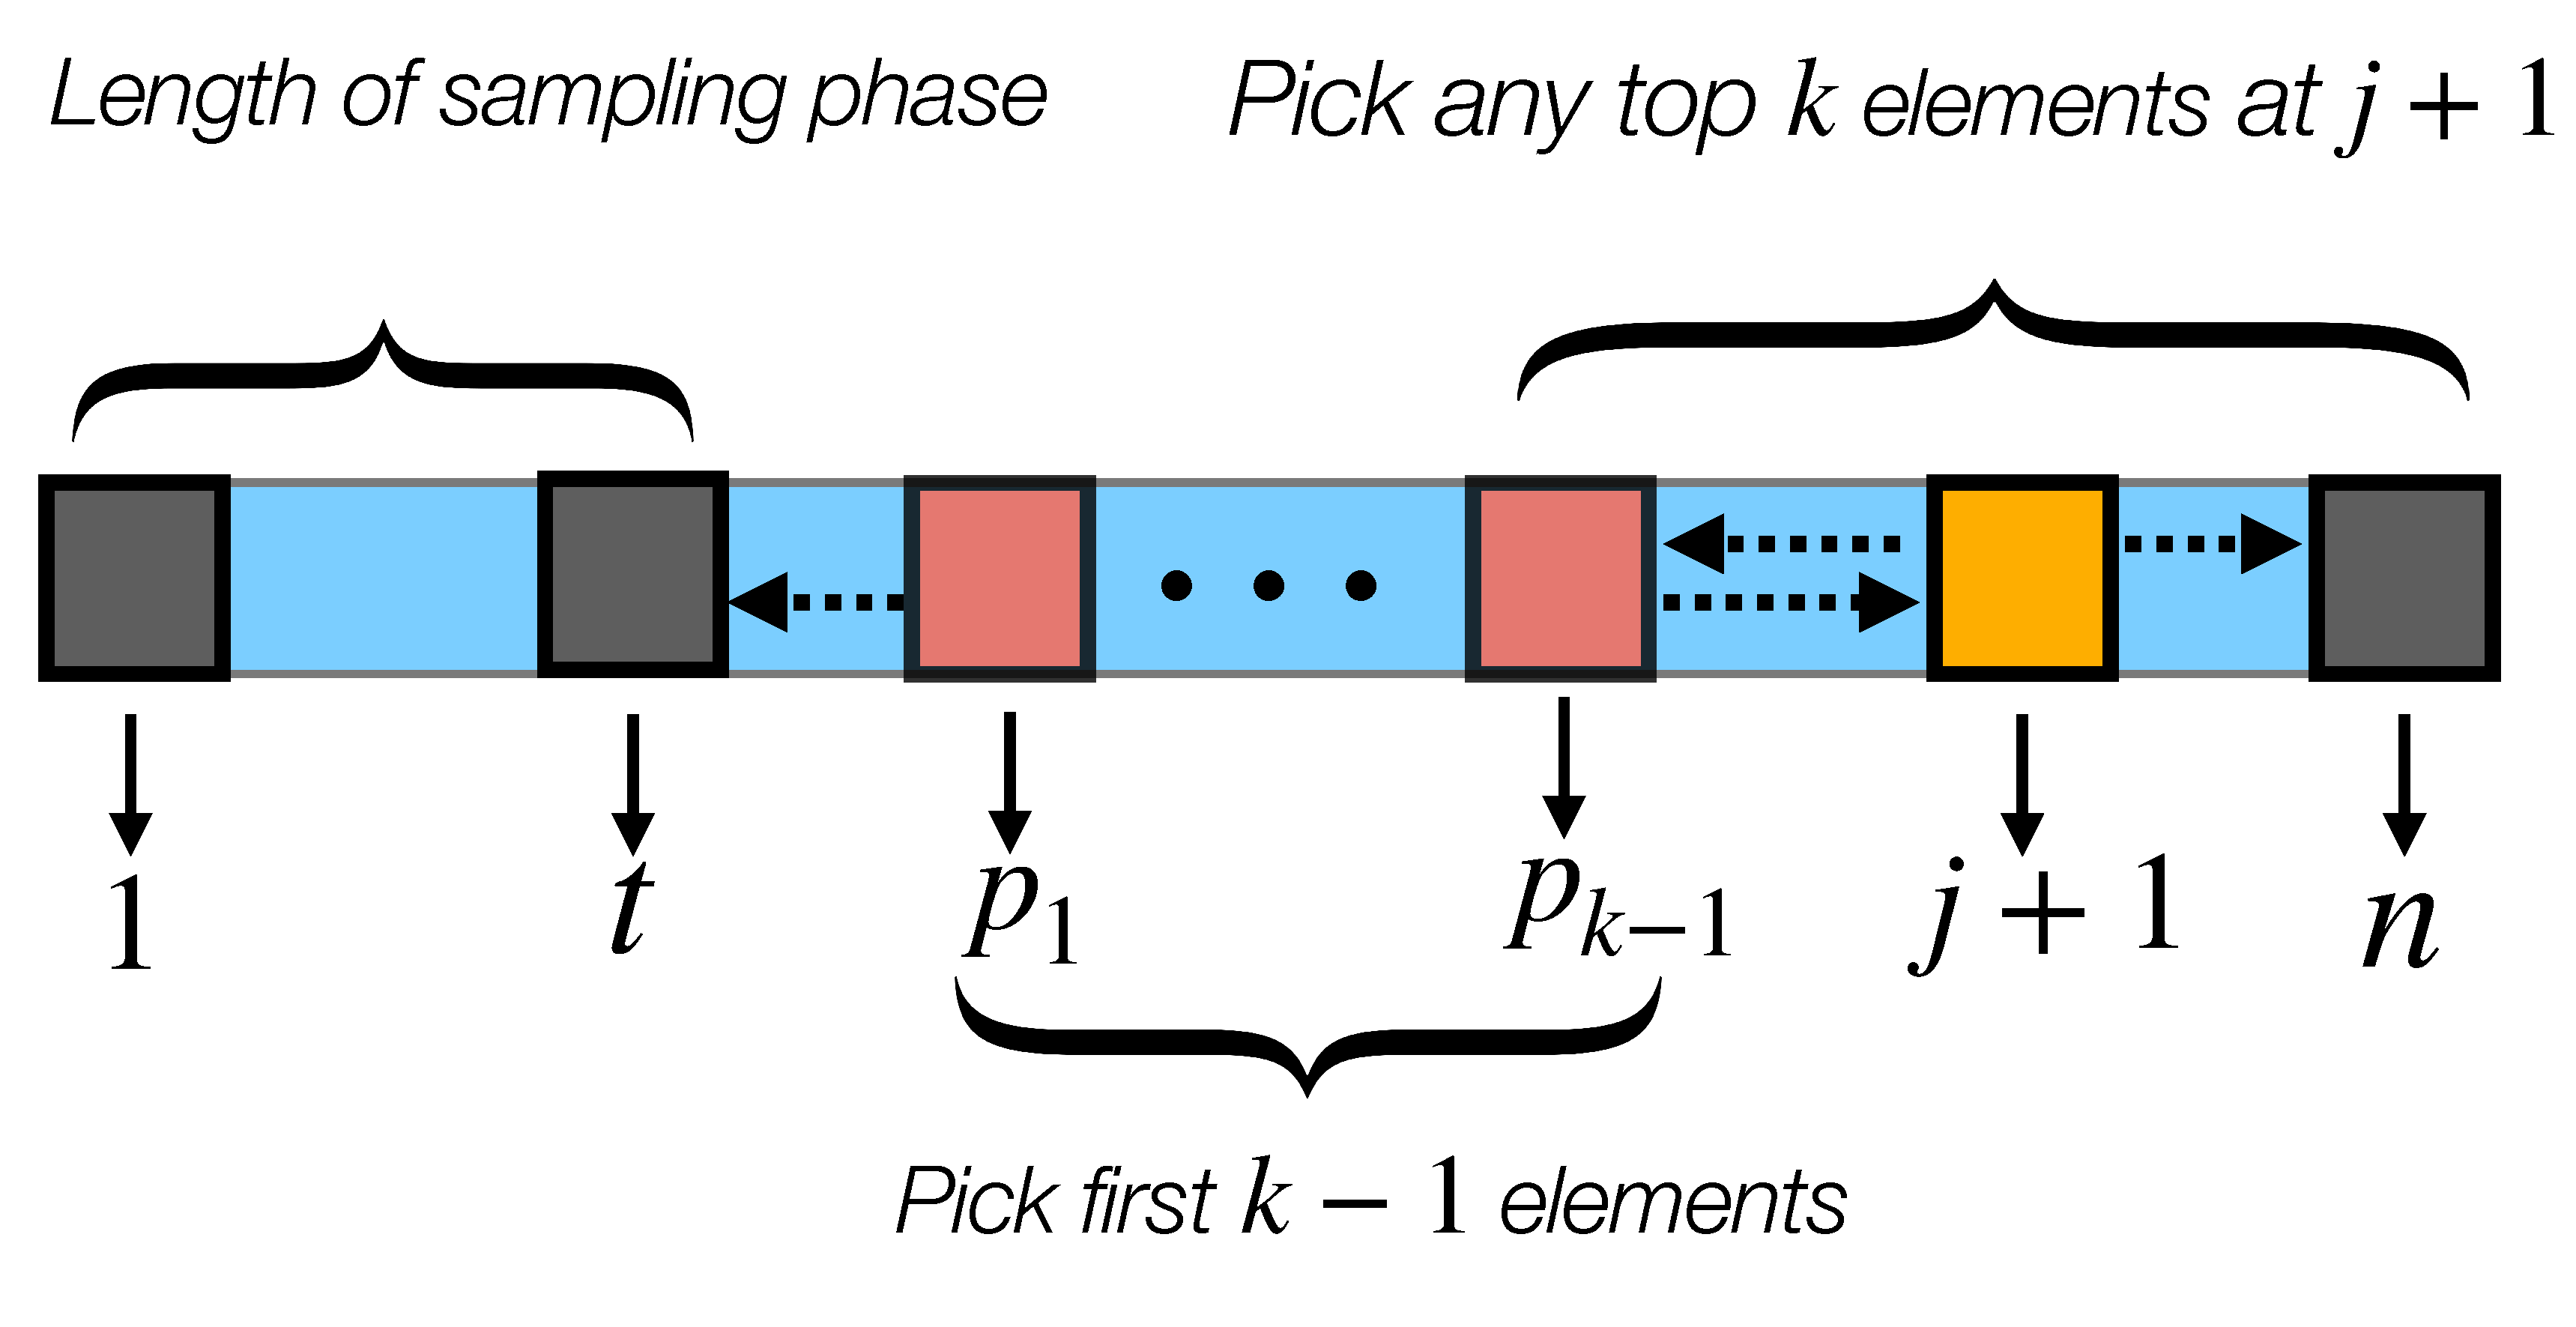
\includegraphics[width=0.50\linewidth]{Figures/virtual_plus_general_k.pdf}
    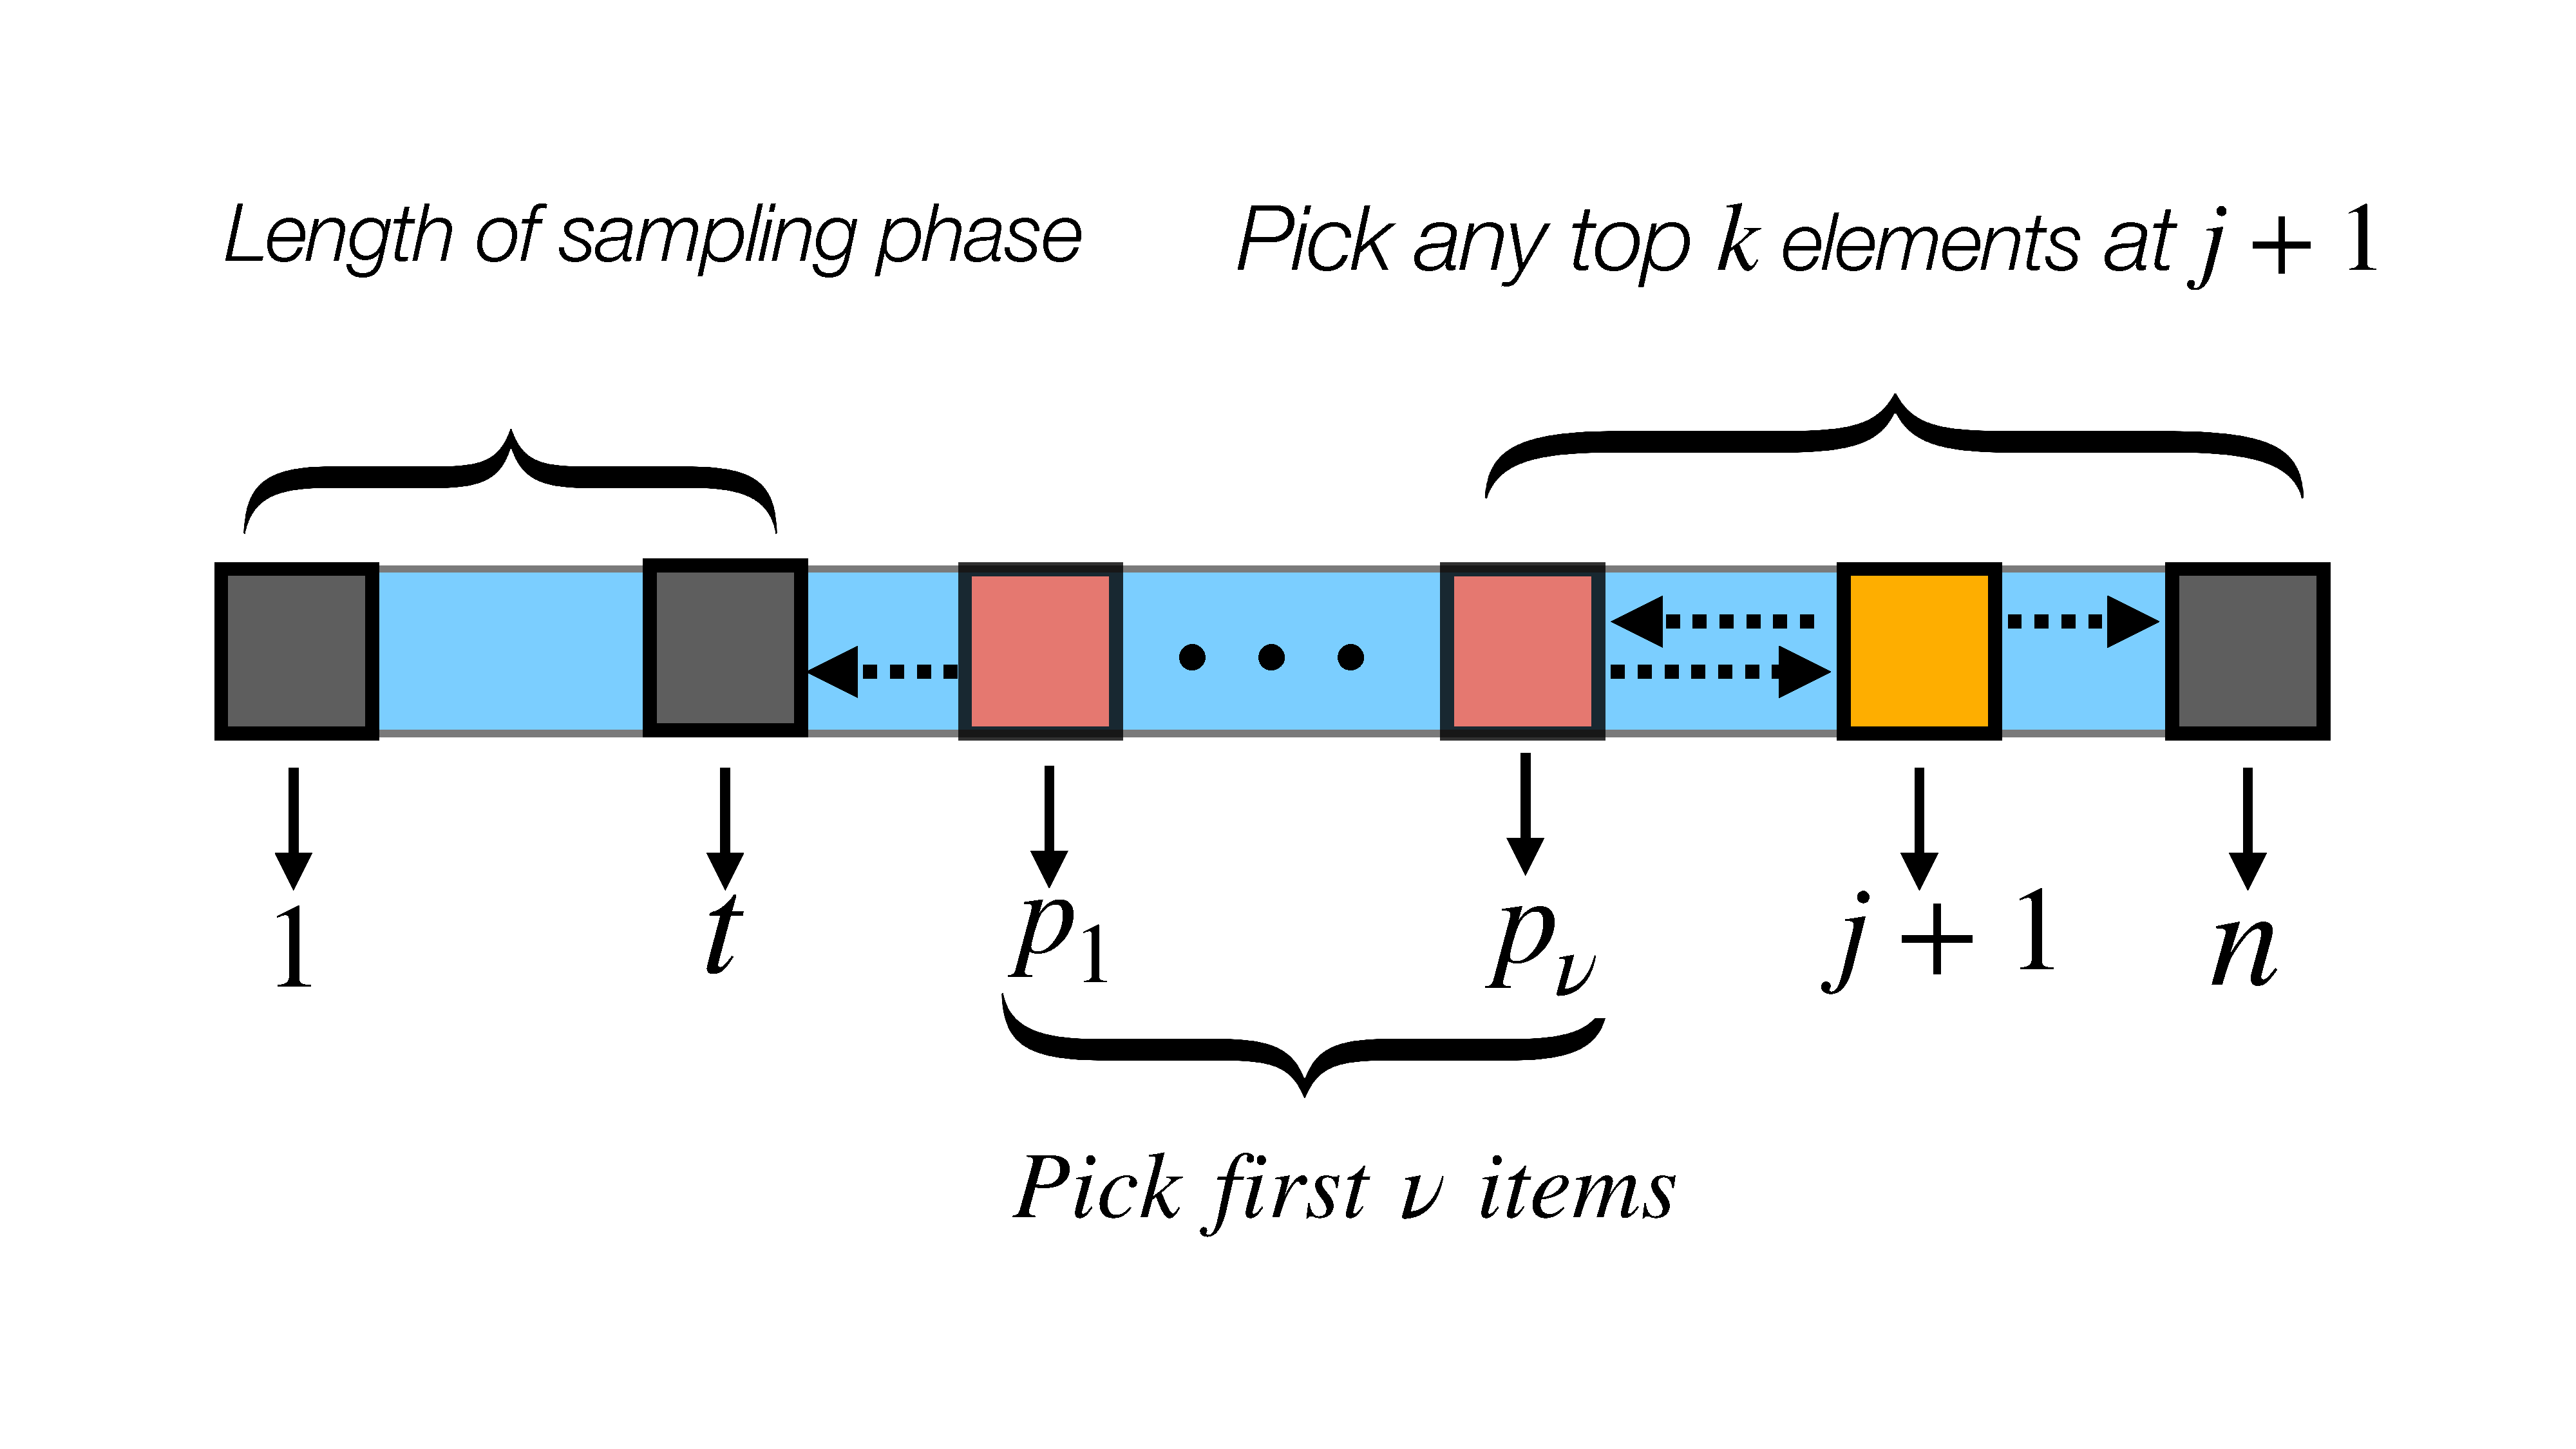
\includegraphics[width=1.0\linewidth]{Figures/general_k.pdf}
    %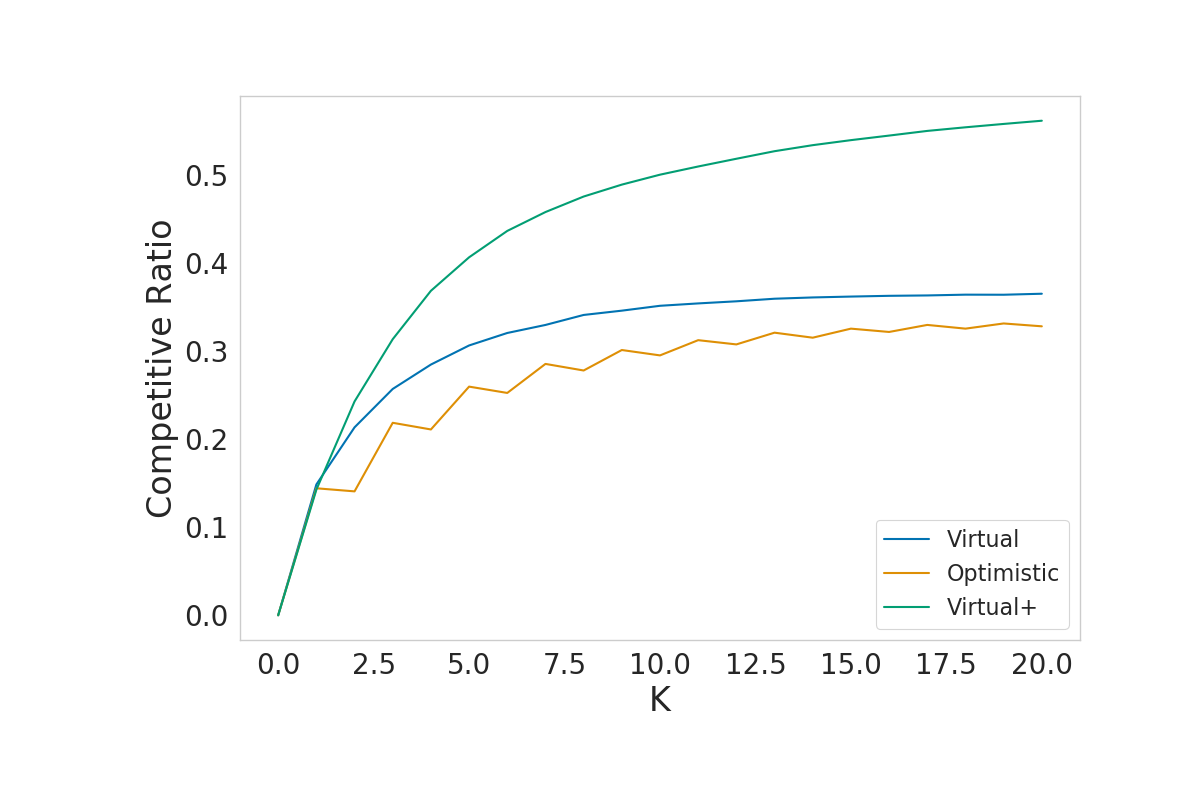
\includegraphics[width=\linewidth]{Figures/Competitive_RatioVar5.png}
    \caption{Virtual+ $k \geq 2$ proof.}
    \label{fig:general_k}
    \vspace{-15pt}
\end{figure}
\begin{proof}
First note that by \citet[Lemma 3.3]{albers2020new} we can show that the competitive ratio for the $k$-secretary problem for a monotone algorithm is equal to 
\begin{equation}
    C = \frac{1}{k}\sum_{a=1}^k \mathbb{P}(i_a \in S_\mathcal{A}), \label{eq:C_as_sum_prob1}
\end{equation}
where $i_a$ is the index of the $a^{th}$ secretary picked by the optimal offline solution ---i.e. $i_a$ is a top-$k$ secretary of $\mathcal{D}$. By Lemma \ref{lemma_monotone} \algoname \ is a monotone algorithm and we may use ~\eqref{eq:C_as_sum_prob1}.

\begin{align}
    \mathbb{P}(i_a \in S_\mathcal{A}) 
    &= \sum_{j=t}^{n-1} \mathbb{P}(i_a \in S_\mathcal{A} \text{ at time-step }j+1) \label{p_picked_equal_not_filled} \\
    &= \frac{1}{n}\sum_{j=t}^{n-1} \mathbb{P}(|S_{\mathcal{A}}| < k \text{ at time-step } j + 1) \notag
\end{align}

Now, we compute $\mathbb{P}(|S_{\mathcal{A}}| < k \text{ at time-step } j+1)$ by decomposing this probability into smaller events  $\mathbb{P}(|S_{\mathcal{A}}| = \nu \text{ at time-step } j+1)$ where $\nu \in [0,\dots,k-1]$.

We may compute the probability of $\mathbb{P}(|S_{\mathcal{A}}| = \nu \text{ at time-step } j+1)$ in the following manner. First, let us consider the scenario where $\nu$ elements are selected by \algoname\ at time steps $p_1$, $p_2, \dots, p_{\nu}$. 
Now, in order for an element to be selected at position $p_\nu$ that element must be one of the top $k$ elements up to time-step $j+1$. Therefore we have a factor $k/j$ in our equation. Now, in order to guarantee that no elements are picked after the position $p_\nu$ we additionally need to ensure that the remaining top-$k$ up to $j+1$ elements appear before $p_\nu$ which results in a factor of ${p_{\nu} - 1 \choose k - 1}/{j-1 \choose k - 1}$. 
Similarly, we may recursively calculate the corresponding factor for each position $p_{\nu-1} \dots p_1$. However, we also need to guarantee that no elements are picked within the time interval $[t+1 \dots p_1-1]$
---i.e. before $p_1$. The probability for this occurring is then ${t \choose k}/{p_1-1 \choose k}$ as this corresponds an ordering where the top-$k$ elements up to $p_1 - 1$ all appear in the sampling phase.
Thus, the probability $p_{t,j}^{k,\nu}:=\mathbb{P}(|S_{\mathcal{A}}| = \nu \text{ at time-step } j+1)$ is :
\begin{align}
    p_{t,j}^{k,\nu}
    &= \sum_{t+1 \leq p_1 < p_2 < \dots <p_{k-1} \leq j}\frac{k}{j} \frac{{p_{\nu} - 1 \choose k-1}}{{j-1 \choose k-1}}\frac{k}{p_{\nu} - 1}
    \frac{{p_{{\nu}-1} - 1 \choose k-1}}{{p_{\nu} - 2 \choose k-1}}\frac{k}{p_{\nu-1} - 1}\dots \frac{k}{p_2 - 1}\frac{{p_1 - 1 \choose k - 1}}{{p_2 - 2 \choose k-1}} \frac{{t \choose k}}{{p_1-1 \choose k}}\\
    & = \frac{t(t-1)\dots(t-k+1)}{j(j-1)\dots (j - k + 1)}\sum_{t+1 \leq p_1 < p_2 < \dots <p_{k-1} \leq j}
    \frac{k^{\nu}}{(p_\nu-k)(p_{\nu-1} - k)\dots(p_1 - k)}
\end{align}

Therefore, the probability of not exceeding $k$-selections, $p_{t,j}^k =\sum_{\nu=0}^{k-1} p_{t,j}^{k,\nu} $, to get before time step $j + 1$ is:
\begin{align}
   \notag
    & \frac{t(t - 1)...(t - k + 1)}{j (j - 1) \dots (j - k + 1)} \bigg(1 + k\hspace{-1em}\sum_{p_1 = t + 1\dots j}^{}\frac{1}{p_1 - k} + \dots
    + {k^{k - 1}}\hspace{-2em}\sum_{\substack{p_1 = t + 1 \dots p_2 - 1  \\\vdots\\ p_{k-1} = t + 1 \dots j}}\frac{1}{(p_1 - k)\dots (p_{k-1} - k)} \bigg)%%\\
    %& = 
    %\frac{t(t - 1)...(t - k + 1)}{j (j - 1) \dots (j - k + 1)} \bigg(1 + k\hspace{-0.5 em}\sum_{p_1 = t + 1}^{j}\frac{1}{p_1 - k} + 
     %\dots  +
     %{k^{k - 1}}\sum_{p_1 = t + 1}^{p_2 -1}\frac{1}{ (p_{1} - k)} \dots \sum_{p_{k-1} = t + 1}^{j}\frac{1}{ (p_{k-1} - k)} \bigg) 
\end{align}
Next, we make use of  
Lemma~\ref{lemma_three}:
\begin{align}
 p_{t,j}^{k} \geq 
     \frac{t(t - 1)\dots (t - k + 1)}{j(j - 1)\dots(j - k + 1)}\left(1 + \frac{k}{1!}\ln \Big(\frac{j - k}{t}\Big) +  \dots + \frac{k^{k - 1}}{(k-1)!}\ln^{k - 1}\Big(\frac{j - k}{t}\Big)\right)
\end{align}
Then we get that the total competitive ratio is: 
\begin{align}
     & \frac{1}{n}\sum_{j = t}^{n - 1}
     \frac{t(t - 1)\dots (t - k + 1)}{j(j - 1)\dots(j - k + 1)}\bigg(1 + \frac{k}{1!}\ln \Big(\frac{j - k}{t}\Big) +  \dots + \frac{k^{k - 1}}{(k-1)!}\ln^{k - 1}\Big(\frac{j - k}{t}\Big)\bigg)\\
     & \geq
     \frac{1}{n}\int_{j = t}^{n}
     \frac{t(t - 1)\dots (t - k + 1)}{j(j - 1)\dots(j - k + 1)}\bigg(1 + \frac{k}{1!}\ln \Big(\frac{j - k}{t}\Big) + \dots + \frac{k^{k - 1}}{(k-1)!}\ln^{k - 1}\Big(\frac{j - k}{t}\Big)\bigg)\\
     & \geq
     \frac{1}{n}\int_{j = t}^{n}
     \frac{t(t - 1)\dots (t - k + 1)}{j^k}\bigg(1 + \frac{k}{1!}\ln \Big(\frac{j - k}{t}\Big) + \dots + \frac{k^{k - 1}}{(k-1)!}\ln^{k - 1}\Big(\frac{j - k}{t}\Big)\bigg)
\end{align}
Now notice that:
\begin{equation}
    \label{identity_two}
    \int\frac{1}{a!} \frac{\ln^a(x)}{x^k} dx = - \frac{1}{x^{k - 1}}\sum_{m = 0}^{a}\frac{1}{m!}(k -1)^{m - 1 -a }\ln^m(x)
\end{equation}
Using the identity in ~\eqref{identity_two} we compute the competitive ratio as:
\begin{align}
     & \geq\frac{t(t - 1)\dots (t - k + 1)}{n}
     \bigg(\sum_{a = 0}^{k - 1}- \frac{1}{j^{k - 1}}{ k ^ a }\sum_{m = 0}^{a}\frac{1}{m!}(k -1)^{m - 1 -a }\ln^m\Big(\frac{j - k}{t}\Big) \bigg) \Big|_{j = t}^{n}\\
     & =
     \frac{t(t - 1)\dots (t - k + 1)}{n}\bigg(- \frac{1}{j^{k - 1}}\sum_{m = 0}^{k - 1}\frac{1}{m!}\Big(\sum_{a = m}^{k - 1}{k ^ a}(k - 1)^{m - a - 1}\Big)\ln^m{\Big(\frac{j - k}{t}\Big)}\bigg)\Big|_{j = t}^{n}
\end{align}
For threshold $t = \alpha n $ where $\alpha \in (0,1)$ and as $n \xrightarrow{}\infty$ our competitive rate becomes:
\begin{align}
    & \alpha \bigg(\sum_{a = 0}^{k - 1}{ k ^ a }{(k - 1)}^{-1 - a}\Big) - \alpha^k\Big(\sum_{m=0}^{k - 1}\frac{1}{m!}\Big(\sum_{a = m}^{k - 1}{ k ^ a }(k - 1)^{m - a - 1}\Big)\ln^m\Big(\frac{1}{\alpha}\Big)\bigg)\\
    & = \alpha\left({\left(\frac{k}{k-1}\right)}^{k} - 1\right) - \alpha^k\left(\sum_{m-0}^{k-1}\left(\frac{\frac{k^k}{(k-1)^{k-m}} - k^m}{m!}\right)(-1)^{m+1}\ln^m(\alpha)\right)
\end{align}
\end{proof}
\begin{definition}
\label{monotone_defn}
An algorithm is called monotone if the probabilities of selecting items $i$ and $j$ satisfy $p_i \geq p_j$ whenever the item values $v_i > v_j$ holds for any two items.
\end{definition}

\begin{lemma}
\label{lemma_monotone}
\algoname \ is a monotone algorithm. 
\end{lemma}
\begin{proof}
    In order to prove that \algoname \ is monotone as defined in Definition \ref{monotone_defn} we must prove that $p_i \geq p_j$ (where $p_i$ is the probability of picking the item $i$) for any two items where $v_i > v_j$. Without loss of generality let us consider a decreasing ordering of $n$-elements based on their values ---i.e. $v_1 > v_{2} > \dots > v_n$. 
    
    
    
    We prove that $p_i \geq p_{i+1}$ for all $i \in [1, \dots, n-1]$ by showing that for each input sequence where $v_{i+1}$ is accepted, there exists a unique input sequence where $v_i$ is accepted. Let us consider a permutation $\pi$ where $v_{i+1}$ appeared and was accepted at time step $a$ while $v_i$ appeared at time step $b$. By swapping $v_i$ and $v_{i+1}$ we obtain a new permutation $\pi'$ where $v_i$ now appears at $a$ and $v_{i+1}$ at $b$. We now study the two following cases.
    
    \xhdr{Case 1: $a < b$}
    
    If $a < b$ notice that the reference set, $R$, and the selected set $S_{\mathcal{A}}$, are exactly the same at time step $a$ for both permutations $\pi$ and $\pi'$. Therefore, if $v_{i+1}$ was accepted at time step $a$ in permutation $\pi$ then $v_i$ will also be accepted at time step $a$ in permutation $\pi'$ since $v_i > v_{i+1}$.   

    \xhdr{Case 2: $a > b$}
    
    If $a > b$ notice that $R$---by definition of \algoname---at time step $a$ contains top-$k$ elements observed in the first $a-1$ time steps. 
    Now the $k$-th element in $R$ at time-step $a$ must satisfy,
    \begin{equation*}
        R^a_{\pi}[k] \geq R^a_{\pi'}[k],
    \end{equation*}
    where $R^a_{[\cdot]}[k]$ corresponds to the $k$-element in the reference set for a specific permutation at time step $a$. Hence, we know that $v_{i} > v_{i+1} \geq R^a_{\pi}[k] \geq R^a_{\pi'}[k]$ as $v_{i+1}$ was assumed to be picked.
    
    
    Furthermore, the $S_{\mathcal{A}}$ and $R$ is the same for permutations $\pi$ and $\pi'$ at time-step $b$. Now by our primary assumption that $v_{i+1}$ is picked at time-step $a>b$ in $\pi$ this means that $v_i$ must be  $v_i \geq R^b_{\pi}[k]$ since $v_i > v_{i+1}$. However, observe that $v_i$ and $R^b_{\pi}[k]$ cannot be consecutive in value as $v_{i+1}$ appears at time-step $a > b$ in permutation $\pi$. This implies that $v_{i+1}$ must also be selected at time step $b$ in permutation $\pi'$ since $v_i$ and $v_{i+1}$ are consecutive in value. By a similar argument based on consecutive order of values between time steps $a$ and $b$ precisely the same elements will be selected in both $\pi$ and $\pi'$. The argument that   $v_{i} > v_{i+1} \geq R^a_{\pi}[k] \geq R^a_{\pi'}[k]$ implies that if $v_{i+1}$ is selected in permutation $\pi$, $v_i$ will also be selected in permutation $\pi'$. The claim then follows by applying the inequality $p_i \geq p_{i+1}$ in an iterative fashion.
\end{proof}
\begin{lemma} 
\label{lemma_three}
Let $f_i \,, \,i = 1 \ldots k$ be decreasing positive functions then we have 
\begin{equation}
    \sum_{p_1=a_1}^{b_1} \ldots \sum_{p_k=a_k}^{p_{k-1}} f_1(p_1) \ldots f_k(p_k)
    \geq \int_{x_1=a_1}^{b_1+1} \ldots \int_{x_k = a_k}^{x_{k-1}+1}  f_1(x_1) \ldots f_k(x_k) dx_1\dots dx_k
\end{equation}
\end{lemma}
\begin{proof}
    The main proof step involves in first noticing that since the functions $f_i \,, \,i = 1 \ldots k$ are decreasing and are positive we have, 
    \begin{equation}
        f_1(p_1) \ldots f_k(p_k) \geq  f_1(p_1) \ldots  f_{k-1}(p_{k-1})\int_{x_k = p_k}^{p_k+1} f_k(x_k) dx_k
    \end{equation}
    Thus, by summing this inequality for $p_k= a_k \ldots p_{k-1}$, we get
    \begin{equation}
    \sum_{p_k=a_k}^{p_{k-1}} f_1(p_1) \ldots f_k(p_k)
    \geq  f_1(p_1) \ldots  f_{k-1}(p_{k-1})  \int_{x_k = a_k}^{p_{k-1}+1} f_k(x_k) dx_k
    \end{equation}
    Now, because the functions $f_i \,, \,i = 1 \ldots k$ are decreasing and positive we have, 
     \begin{align}
    \mathcal{S} 
    &= \sum_{p_k=a_k}^{p_{k-1}} f_1(p_1) \ldots f_k(p_k)\\
    &\geq  f_1(p_1) \ldots  f_{k-2}(p_{k-2})  \int_{x_{k-1} = p_{k-1}}^{p_{k-1}+1} f_{k-1}(x_{k-1})  \int_{x_k = a_k}^{p_{k-1}+1} f_k(x_k) dx_{k-1}dx_k \\
    &\geq f_1(p_1) \ldots  f_{k-2}(p_{k-2})  \int_{x_{k-1} = p_{k-1}}^{p_{k-1}+1} f_{k-1}(x_{k-1})  \int_{x_k = a_k}^{x_{k-1}} f_k(x_k) dx_{k-1}dx_k 
    \end{align}
    where for the last inequality we used the fact that $x_{k-1} \in [p_{k-1}, p_{k-1}+1]$.
    Finally, by summing for $p_{k-1} = a_{k-1} \ldots p_{k-2}$, we get,
    \begin{align}
    \sum_{p_{k-1}=a_{k-1}}^{p_{k-2}}\mathcal{S} &= \sum_{p_{k-1}=a_{k-1}}^{p_{k-2}} \sum_{p_k=a_k}^{p_{k-1}} f_1(p_1) \ldots f_k(p_k)\\
    &\geq f_1(p_1) \ldots  f_{k-2}(p_{k-2})  \int_{x_{k-1} = p_{k-1}}^{p_{k-1}+1} f_{k-1}(x_{k-1})  \int_{x_k = a_k}^{x_{k-1}} f_k(x_k) dx_{k-1}dx_k
    \end{align}
    Using a recursive argument we finally get,
    \begin{equation}
    \sum_{p_1=a_1}^{b_1} \ldots \sum_{p_k=a_k}^{p_{k-1}} f_1(p_1) \ldots f_k(p_k)
    \geq \int_{x_1=a_1}^{b_1+1} \ldots \int_{x_k = a_k}^{x_{k-1}+1}  f_1(x_1) \ldots f_k(x_k) dx_1\dots dx_k
\end{equation}
\end{proof}


\clearpage
\subsection{Analytic computation of $C_k$ for \algoname}

\begin{table}[ht!]
    \centering
    \caption{Values of the Competitive ratio $C_k$ and the associated optimal $\alpha_k$ needed to compute the threshold for \algoname. Note that for $5\leq k\leq 100$ the competitive ratio of \textsc{Single-Ref} provided by~\citet{albers2020new} outperforms \algoname's competitive ratio. However, our analysis provides a tractable way to scale the analytic computation of the competitive ratio with $k$ as the function to optimize (and its gradients) in Theorem~\ref{thm:general_k_theorem1} is $\mathcal{O}(k)$.}
    \vspace{2pt}
    \begin{tabular}{ccccccccccc}
     \toprule
          $k$ & 2 &3 & 4 & 5 & 100 & 200 &300 &400 & 500 & 600\\
         \midrule
        $C_k$ & .4273&.4575&.4769&.4906&.5959&.6062&.6108&.6136&.6156&.6170 \\
        $\alpha_k$ & .3824 &.3867&.3884&.3890&.3781 &.3755 &.3743&.3735&.3729&.3726 \\
        \bottomrule
    \end{tabular}
    \label{tab:C_k}
\end{table}

\section{Proof of Theorem~\ref{thm:stochastic_secretary}}
\label{appendix:proof_thm2}
We now prove Theorem \ref{thm:stochastic_secretary} in detail, reproduced here for convenience. 

\begin{reptheorem}{thm:stochastic_secretary}
Let $\mathcal{A}$ be a $C$-competitive secretary algorithm that observes independent random variables $\mathcal{V}_{i},\, i\in [n]$ satisfying Eq.~\ref{eq:concentration}. If $\Delta = \tfrac{1}{2}\min_{1\leq i \neq j \leq  n } |v_i - v_j|$ is positive, then $\mathcal{A}$ has a non-vanishing stochastic competitive ratio $C_{s}$ of at least:  
\begin{equation}
    C_n \left( 1-e^{- \frac{\Delta}{2 \sigma^2}} \right)^{\left(-2 \exp(- \frac{\Delta}{2 \sigma^2})\right)/\left({1 -  \exp(\frac{-\Delta}{\sigma^2})}\right)}
   % {\frac{-2 \exp(- \frac{\Delta}{2 \sigma^2})}{1 -  \exp(\frac{-\Delta}{\sigma^2})}}
\end{equation}
\end{reptheorem}

\begin{proof}
In this analysis, we will refer to the deterministic online algorithm as $\mathcal{A}$. Please note, the following statement of results holds for \textit{any} online algorithm. As a result, when introducing certain lemmas we will use algorithm $\mathcal{A}$ as a general single threshold deterministic secretary algorithm and not any specific one. Furthermore, we will denote the stochastic versions of $\mathcal{A}$ as $\mathcal{A}^{s}$.
Let $v_1^*, v_2^*, \dots v_k^*$ be the values of top $k$ elements and let $i_1^*, i_2^* \dots i_k^*$ be their appropriate indices. Therefore, the optimal offline solutions selects set 
$S^* = \{i_1^*, i_2^*, \dots i_k^*\}$, while a deterministic online algorithm $\mathcal{A}$ in the stochastic setting chooses set $S$, and our online algorithm $\mathcal{A}^{s}$ chooses set $S^{(s)}$. Our goal is to provide a lower bound of the kind
\begin{equation}
     \frac{\mathbb E[|S^{(s)} \cap S^*|]}{k} \geq c\frac{\mathbb E[|S \cap S^*|]}{k}
\end{equation}
where $c>0$ is a constant that depends on the randomness of the estimates $\mathcal{V}_i\,,i=1,\ldots,n.$ 
Assuming that $\mathcal{A}$ is $C_n$-optimal, this lower bound will provide us a competitive ratio for the stochastic algorithm $\mathcal{A}^{s}$.

% 
% Note that for any two random variable $X_i$ and $X_j$ for which we know that $\omega_i > \omega_j$ holds:
% \begin{align*}
% \sP(X_i < X_j)  & = 
% \sP((X_i - \omega_i) - (X_j - \omega_j) < \omega_j - \omega_i)  \\ & =   \sP (\epsilon_i - \epsilon_j < -\Delta) \leq e^{\frac{-\Delta}{{2\sigma}^2}}
% \end{align*}
%  therefore
%  \begin{equation}\label{equ:eight}
%  \sP(X_i > X_j) \geq (1 -  e^{\frac{-\Delta}{{2\sigma}^2}})
% \end{equation}


Now, by definition the algorithm $\mathcal{A}^{s}$ is the online algorithm $\mathcal{A}$ but operating on the random variables $\mathcal{V}_1, \mathcal{V}_2, ...\mathcal{V}_n$ (instead of $v_1,\ldots, v_n$). Thus, we call $i_a^{(s)}$ the index of the $a$ largest value among  $\mathcal{V}_1, \mathcal{V}_2, ...\mathcal{V}_n$ (note that $i_a^{(s)}$ is a random variable) and we have that 
\begin{equation}
   \sP[i_a^* \in S] = \sP[i_a^{(s)} \in S^{(s)}|\mathcal{V}_1, \dots,\mathcal{V}_n],
\end{equation}
by summing over $a$ and taking an expectation over all permutations while noting $\{i_1^{(s)},\ldots,i_k^{(s)}\} := S^*_s$
\begin{equation}
    \sE[|S^* \cap S|] = \sE[|S^*_s \cap S^{(s)}|  \; | \mathcal{V}_1, \ldots,\mathcal{V}_n]
\end{equation}
Now it is easy to see that the expected number of indices in $S^*$ picked by $\mathcal{A}^{s}$ is larger than the expected number of indices in $S^*_s\cup S^*$. Formally,
\begin{align}
    \sE[|S^* \cap S^{(s)}|]  \notag
    &\geq \sE[|S^* \cap S^{(s)} \cap S^*_s|] \notag \\
    &\geq \sE [ \mathbf{1}\{S^* = S^*_s\} \sE[|S^* \cap S^*_s|\,| \mathcal{V}_1, \ldots,\mathcal{V}_n]] \notag\\
    &= \sP(S^*=S^*_s) \sE[|S^* \cap S|].
\end{align}
% \begin{equation}
%      \sum_{a=1}^k \sP[i_a^* \in S^{(s)}]
%      \geq \sum
%      _{a=1}^k \sP[i_a^{(s)} \in S^{(s)} \text{ and } i_a^{(s)} \in S^*]
% \end{equation}
Without loss of generality we can consider an ordering over true values $v_1 \geq \dots \geq v_n$. Also, let us denote $\bar v:= \frac{v_k + v_{k+1}}{2}$. If we consider the event $\mathcal{V}_{i_a^*} \geq \bar v \geq \mathcal{V}_{i_b^*}$ for $1 \leq a \leq k < b \leq n$ then $S^*=S^*_s$. Let us formally bound the probability of the event  $S^*=S^*_s$,
\begin{align*}
    \sP(S^*=S^*_s) 
    &\geq \sP(\mathcal{V}_{i_1^*}, \ldots, \mathcal{V}_{i_k^*} \geq \ldots \geq \mathcal{V}_{i_{k+1}^*} , \ldots, \mathcal{V}_{i_n^*})  \\
     & \geq \sP(\mathcal{V}_{i_a^*} \geq \bar v \geq \mathcal{V}_{i_b^*}\,,\,1 \leq a \leq k < b \leq n) \\
    & \geq \sP(\mathcal{V}_{i_a^*} \geq v_a - (2(k-a)+1)\Delta\,,\,   v_b + (2(b-k)-1) \Delta \geq  \mathcal{V}_{i_b^*}\,,\,1 \leq a \leq k < b \leq n) \\
\end{align*}
where in the last inequality we used $\Delta = \tfrac{1}{2}\min_{1\leq i \neq j \leq  n } \{\mid v_i - v_j \mid \}
$. Thus we have
\begin{equation}
    v_a - (2(k-a)+1)\Delta \geq \bar v \geq  v_b + (2(b-k)-1) \Delta \,, \quad \forall \, 1 \leq a \leq k < b \leq n \,.
\end{equation}
Finally, using the fact that the random variables $\mathcal{V}_i$ are independents we have,
\begin{align*}
    \sP(S^*=S^*_s)      
    & \geq \sP(|\mathcal{V}_{i_a^*} - v_a| \leq  2|k+1/2-a|\Delta, \,a \in [n]) \\
    & = \prod_{a=1}^n \sP(|\mathcal{V}_{i_a^*} - v_a| \leq  2|k+1/2-a|\Delta) \\
    & \geq \prod_{i=1}^n  (1 - e^{\frac{-2|k+1/2-i|\Delta}{2\sigma^2}})
\end{align*}
Where the last inequality comes from the assumption that 
\begin{equation}
    \sP( |\mathcal{V}_i-v_i| \geq \epsilon) \leq e^{\frac{-\epsilon^2}{2\sigma^2}} \,,\,\forall i \in [n]\,.
\end{equation}

Finally, we can lower-bound $\sum_{i=1}^n\log (1 - e^{\frac{-2|k+1/2-i|\Delta}{2\sigma^2}})$ by leveraging the concavity of $\log$ for any $x$ in $0<x<a<1$, %we have by concavity of the $\log$,
\begin{equation}
    \log(1-x) \geq \log(1-a) x \,.
\end{equation}
Thus,
\begin{align}
    \sum_{l=1}^n\log (1 - e^{\frac{-2|k+1/2-l|\Delta}{2\sigma^2}}) 
    & \geq \log(1-e^{- \frac{\Delta}{2 \sigma^2}}) \sum_{l=1}^n e^{\frac{-2|k+1/2-l|\Delta}{2\sigma^2}} \\
    & \geq -2\log(1-e^{- \frac{\Delta}{2 \sigma^2}}) e^{- \frac{\Delta}{2 \sigma^2}} \sum_{l=1}^{\infty} e^{\frac{-l\Delta}{\sigma^2}} \\
    & \geq -2\log(1-e^{- \frac{\Delta}{2 \sigma^2}}) \frac{e^{- \frac{\Delta}{2 \sigma^2}} }{1 -  e^{\frac{-\Delta}{\sigma^2}}}
\end{align}
Which finally gives us,
\begin{equation}
     \sP(S^*=S^*_s)    \geq \left( 1-e^{- \frac{\Delta}{2 \sigma^2}} \right)^{\left(-2 \exp(- \frac{\Delta}{2 \sigma^2})\right)/\left({1 -  \exp(\frac{-\Delta}{\sigma^2})}\right)}
\end{equation}



Note that we could refine this bound by considering individual gaps $\Delta_i$ and constants $\sigma_i$ and consider $\frac{\Delta}{\sigma^2} = \min_{i \in [n]} \frac{\Delta_i}{\sigma_i}$.

\end{proof}


\clearpage


\section{Classical Online Algorithms for Secretary Problems}
\label{appendix:classical_online_algorithms}

All single threshold online algorithm described in this paper include: \textsc{Virtual}, \textsc{Optimistic} and \textsc{Single-Ref}. Each online algorithm consists of two phases ---\textbf{sampling phase} followed by \textbf{selection phase}--- and an optimal stopping point $t$ which is used by the algorithm to transition between the phases. We now briefly summarize these two phases for the aforementioned online algorithms. 

\xhdr{Sampling Phase - \textsc{Virtual}, \textsc{Optimistic} and \textsc{Single-Ref}}
In the sampling phase, the algorithms passively observe all data points up to a pre-specified time index $t$, but also maintains a sorted reference list $R$ consisting of the $k$ elements with the largest values $\mathcal{V}(i)$ seen. Thus the $R$ contains a list of elements sorted by decreasing value. That is $R[k]$ is the index of the $k$-th largest element in $R$ and $\mathcal{V}(R[k])$ is its corresponding value. The elements in $R$ are kept for comparison but are crucially \textit{not} selected in the sampling phase.

\subsection{\textsc{Virtual} Algorithm}

\xhdr{Selection Phase - \textsc{Virtual} algorithm}
Subsequently, in the selection phase, $i > t$, when an item with value $\mathcal{V}(i)$ is observed an irrevocable decision is made of whether the algorithm should select $i$ into $S$. To do so, the Virtual algorithm simply checks if the value of the $k$-th smallest element in $R$, $\mathcal{V}(R[k])$, is smaller than $\mathcal{V}(i)$ in addition to possibly updating the set $R$. The full Virtual algorithm is presented in Algorithm 1.

\begin{algorithm}[ht]
\textbf{Inputs:} $t\in[k\dots n-k]$, $R = \emptyset$, $S_{\mathcal{A}} = \emptyset$
\newline
\textbf{Sampling phase:} Observe the first $t$ data points and construct a list $R$ with the indices of the top $k$ data points seen.  $\texttt{sort}$ ensures: $ \mathcal{V}(R[1]) \geq \mathcal{V}(R[2]) \dots \geq \mathcal{V}(R[k]).$

\textbf{Selection phase (at time $i>t$):}

\begin{algorithmic}[1]
\IF {$ \mathcal{V}(i) \geq  \mathcal{V}(R[k])$
and $R[k] > t$} 
        \STATE $R$ = $\texttt{sort}\{R \cup \{i\} \setminus \{R[k]\}\}$ \hfill\COMMENT{// Update $R$ with element $i$ and also take out $R[k]$}
\ELSIF{ $ \mathcal{V}(i) \geq  \mathcal{V}(R[k])$
and $R[k] \leq t$}
        \STATE $R$ = $\texttt{sort}\{R \cup \{i\} \setminus \{R[k]\}\}$ \hfill\COMMENT{// Update $R$ with element $i$ and also take out $R[k]$}
        \STATE $S_\mathcal{A} = \{ S_\mathcal{A} \cup \{i \}\}$ \hfill\COMMENT{// Select element $i$}
\ENDIF 
\STATE
$i\gets i + 1$
\end{algorithmic}
 \caption{\textsc{Virtual Algorithm}}
\end{algorithm}


\subsection{\textsc{Optimistic} Algorithm}

\xhdr{Selection Phase - \textsc{Optimistic} algorithm}
In the optimistic algorithm, i is selected if and only if $\mathcal{V}(i) \geq \mathcal{V}(R[last])$. Whenever $i$ is selected, $R[last]$
is removed from the list
$R$, but no new elements are ever added to $R$. Thus, intuitively, elements are selected when they beat one of the remaining reference
points from $R$.
We call this algorithm “optimistic” because it removes the reference
point $R[last]$ even if $ \mathcal{V}(i)$ exceeds, say, $ \mathcal{V}(R[1])$. Thus, it implicitly assumes
that it will see additional very valuable elements in the future, which
will be added when their values exceed those of the remaining, more
valuable, $R[a]\,,\,a \in [k]$.


\begin{algorithm}[ht]
\textbf{Inputs:} $t\in[k\dots n-k]$, $R = \emptyset$, $S_{\mathcal{A}} = \emptyset$.

\textbf{Sampling phase (up to time $t$):} Observe the first $t$ data points and construct a list $R$ with the indices of the top $k$ data points seen. $\texttt{sort}$ ensures: $ \mathcal{V}(R[1]) \geq \mathcal{V}(R[2]) \dots \geq\mathcal{V}(R[k]).$
Set $last = k$, to be the index of the last element in $R$.

\textbf{Selection phase (at time $i>t$):}

\begin{algorithmic}[1]
\IF {$\mathcal{V}(i) \geq \mathcal{V}(R[last])$} 
        \STATE $R$ = $\{R \setminus \{R[last]\}\}$ \hfill\COMMENT{// Update $R$ by taking out $R[k]$}
        \STATE $S_\mathcal{A} = \{ S_\mathcal{A} \cup \{i \}\}$ \hfill\COMMENT{// Select element $i$}
        \STATE $last = last - 1$
\ENDIF 
$i\gets i + 1$
\end{algorithmic}
 \caption{\textsc{Optimistic Algorithm}}
\end{algorithm}

\subsection{\textsc{Single-Ref} Algorithm}
\xhdr{Selection Phase - \textsc{Single-Ref} algorithm}
In the \textsc{Single-Ref} algorithm, $i$ is selected if and only if $\mathcal{V}(i) \geq \mathcal{V}(R[r])$ and we haven't already selected $k$ elements. 
We call this algorithm single reference algorithm because we always compare incoming elements to one single reference element, that was determined in the sampling phase.

\begin{algorithm}[ht]
\textbf{Inputs:} $t\in[k\dots n-k]$, $R = \emptyset$, $S_{\mathcal{A}} = \emptyset$, $r \in [k]$ (reference rank)

 \textbf{Sampling phase (up to time $t$):} Observe the first $t$ data points and construct a list $R$ with the indices of the top $k$ data points seen. Let $s_r = R[r]$ be the $r$-th best item from the sampling phase.

\textbf{Selection phase (at time $i>t$):} 
\begin{algorithmic}[1]
\IF {$\mathcal{V}(i) \geq s_r$ and $ |S_{\mathcal{A}}| \leq  k$} 
        \STATE $S_\mathcal{A} = \{ S_\mathcal{A} \cup \{i \}\}$ \hfill\COMMENT{// Choose the first $k$ items better than $s_r$}

\ENDIF 

$i\gets i + 1$
\end{algorithmic}
 \caption{\textsc{Single-Ref Algorithm}}
\end{algorithm}

\clearpage
\section{Additional Experimental Results}
\label{appendix:additional_results}

\subsection{Additional Results on Synthetic Data}
\label{appendix:synthetic_additional_results}
We now provide additional results on Synthetic Data with varying levels of noise added to each item in $\mathcal{D}$. In particular, we investigate in figure \ref{fig:additional_results_synthetic_data} online algorithms in the face of no noise ---i.e. $\sigma^2 = 0$, $\sigma^2 = 1$, and $\sigma^2 = 5$ in addition to $\sigma^2 = 10$ reported in figure \ref{fig:synthetic_data}. The deterministic setting corresponds to $\sigma^2 = 0$ while $\sigma^2=1$ and $\sigma^2=1$ correspond to the stochastic setting as introduced in section \ref{stochastic_k_secretary}.

\begin{figure}[ht]
    \centering
    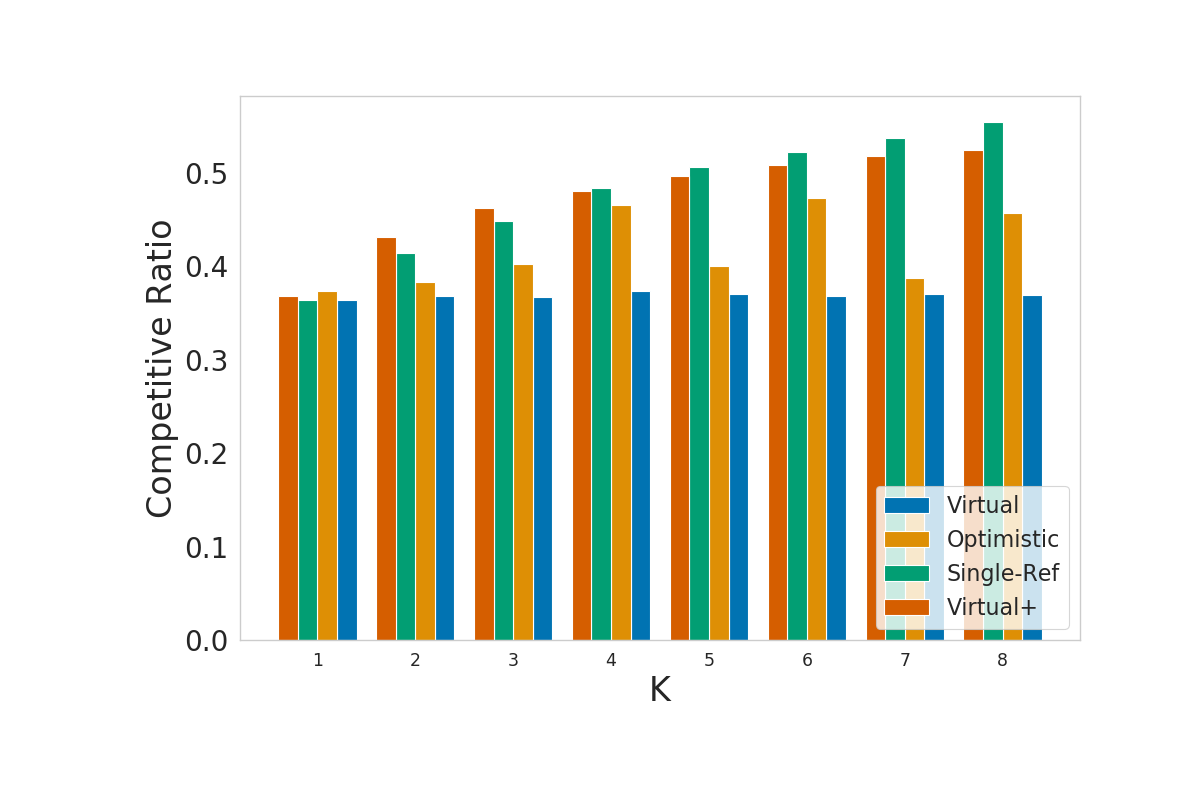
\includegraphics[width=0.32\linewidth]{Figures/Competitive_RatioBar8-Deterministic.png}
    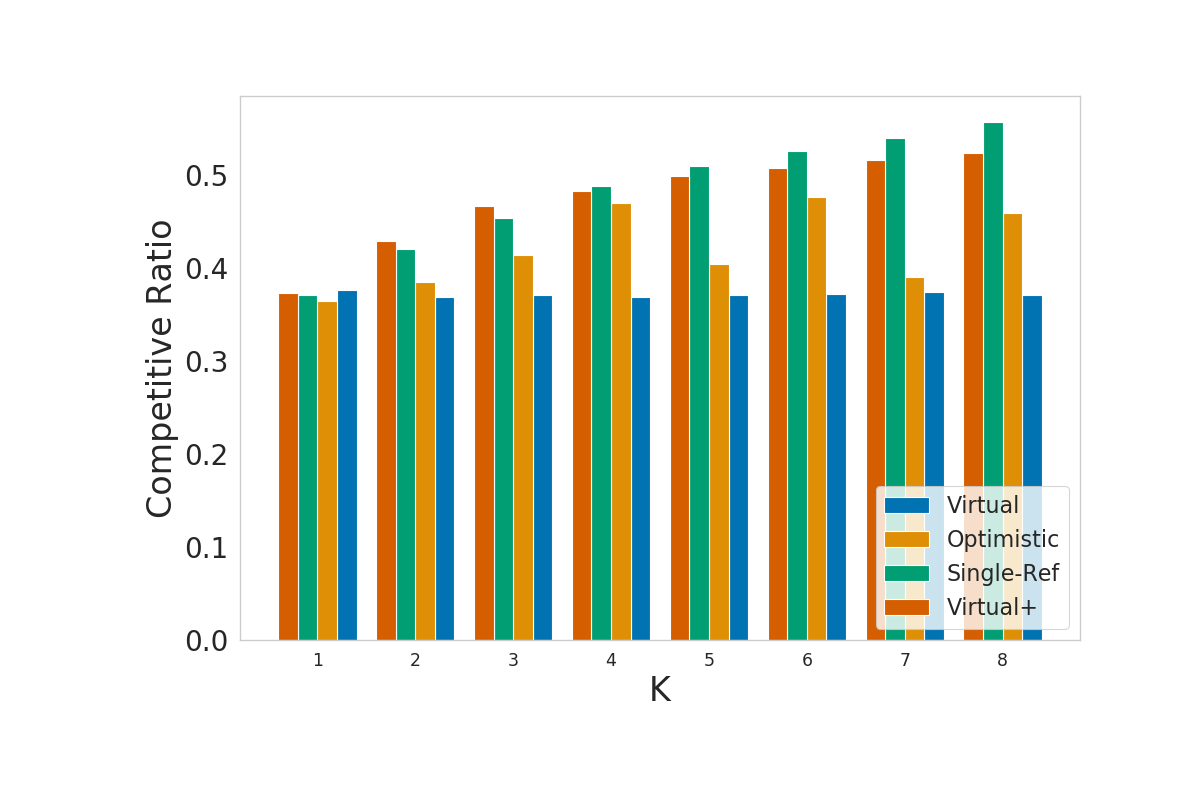
\includegraphics[width=0.32\linewidth]{Figures/Competitive_RatioBar8-Var-1.png}
    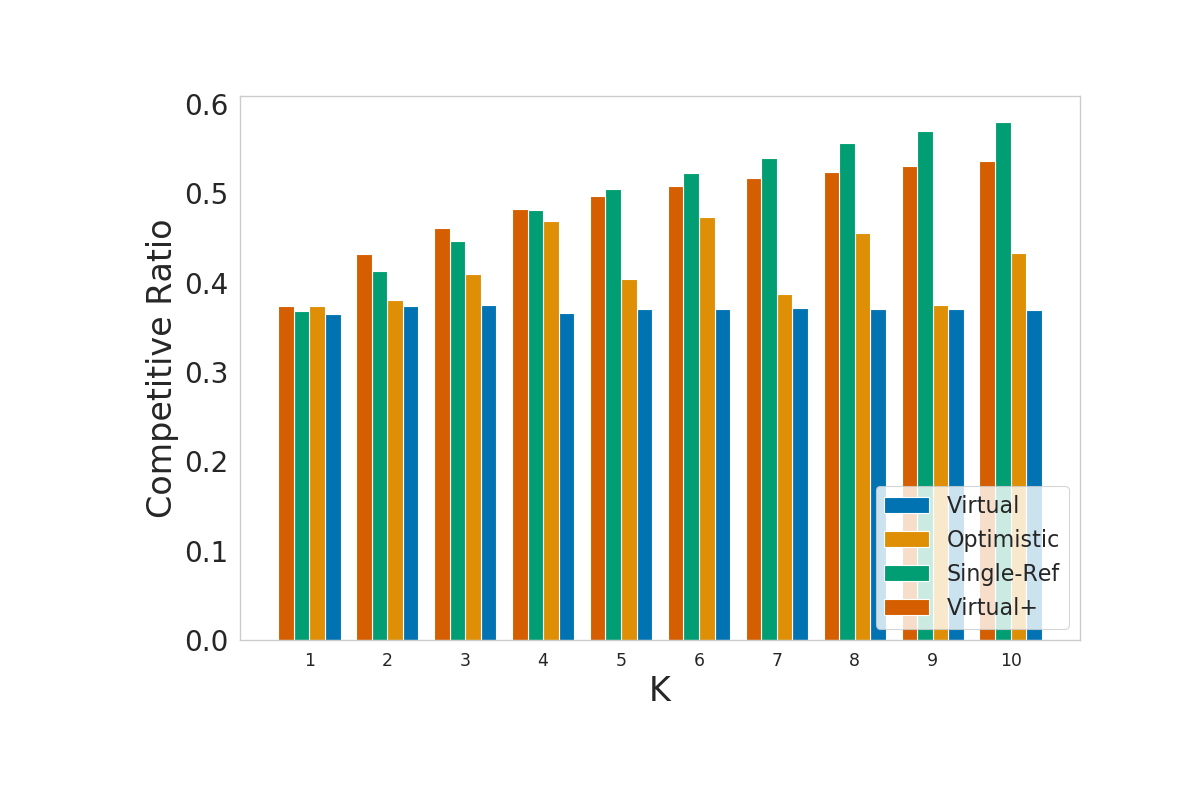
\includegraphics[width=0.32\linewidth]{Figures/Competitive_RatioBar-Var-5.png}
    \caption{Estimation of the competitive ratio of online algorithms under various noise levels. \textbf{Left:} Deterministic setting with $\sigma^2=0$. \textbf{Middle:} Stochastic setting with $\sigma^2 = 1$. \textbf{Right:} Stochastic setting with $\sigma^2 = 5$.}
    \label{fig:additional_results_synthetic_data}
\end{figure}




\subsection{Experimental Details}
\label{appendix:additional_results_larger_datasets}
We provide more details about the experiments presented in section~\ref{section:experiments}. For further details we also invite the reader to look at the code provided with the supplementary materials.

\paragraph{Attack strategies} We use two different attack strategies the Fast Gradient Sign Method (FGSM) \citep{goodfellow2014explaining} and 40 iterations of the PGD attack \citep{madry2017towards} with $l_\infty$.

\paragraph{Hyper-parameters of online algorithms} All the online algorithms except \textsc{Single-Ref} have a single hyper-parameters to choose which is the length of the sampling phase $t$. For \textsc{Virtual} and \textsc{Optimistic} we use $t=\floor{ \frac{t}{e}}$ which is the value suggested by theory in \citet{babaioff2007knapsack}. For \algoname \ we use $t=\alpha n$  as found by solving the maximization problem for a specific $k$ in Theorem~\ref{thm:general_k_theorem1}. \textsc{Single-Ref} has two hyper-parameters to choose the threshold $t$ ($c$ in the original paper) and reference rank $r$. For $k=1...100$ the values are given in \citet{albers2020new} and are numerical solutions to combinatorial optimization problems. However, for $k = 1000$ no values are specified and we choose $c=0.13$ and $r=40$ through grid search. Indeed, these values may not be optimal ones but we leave the choice of better values as future work.

\paragraph{MNIST model architectures} For table~\ref{table:non_robust_table1}, $f_s$ and $f_t$ are chosen randomly from an ensemble of trained classifiers. The ensemble is composed of five different architectures described in table~\ref{appendix:mnist_ens_adv_training_table}, with 5 trained models per architecture.

\begin{table}[h]
    \centering
          
            \begin{tabular}{ccccc}
            \toprule
                   &  A  & B  & C & D \\
                    \midrule
                   & Conv(64, 5, 5) + Relu & Dropout(0.2) & Conv(128, 3, 3) + Tanh & \multirow{2}{*}{\shortstack{FC(300) + Relu \\ Dropout(0.5)}}\\
                   & Conv(64, 5, 5) + Relu &  Conv(64, 8, 8) + Relu &  MaxPool(2,2) & \\
                   & Dropout(0.25) & Conv(128, 6, 6) + Relu  & Conv(64, 3, 3) + Tanh & \multirow{2}{*}{\shortstack{FC(300) + Relu \\ Dropout(0.5)}} \\
                   & FC(128) + Relu & Conv(128, 6, 6) + Relu & MaxPool(2,2) & \\
                   & Dropout(0.5) &  Dropout(0.5)  &  FC(128) + Relu &  \multirow{2}{*}{\shortstack{FC(300) + Relu \\ Dropout(0.5)}}\\
                   & FC + Softmax &  FC + Softmax &  FC + Softmax & \\
                   & & & & \multirow{2}{*}{\shortstack{FC(300) + Relu \\ Dropout(0.5)}} \\
                   & & & & \\
                   & & & & FC + Softmax \\
            \bottomrule
            \end{tabular}
            \caption{The different MNIST Architectures used for $f_s$ and $f_t$}
            \label{appendix:mnist_ens_adv_training_table}
    \end{table}

\paragraph{CIFAR model architectures} For table~\ref{table:non_robust_table1}, $f_s$ and $f_t$ are chosen randomly from an ensemble of trained classifiers. The ensemble is composed of five different architectures: VGG-16 \citep{simonyan2014very}, ResNet-18 (RN-18) \citep{he2016deep}, Wide ResNet (WR) \citep{zagoruyko2016wide}, DenseNet-121 (DN-121) \citep{huang2017densely} and Inception-V3 architectures (Inc-V3) \citep{szegedy2016rethinking}, with 5 trained models per architecture.

\subsection{Additional metrics}
In addition to the results provided in table~\ref{table:non_robust_table1}, we also provide two other metrics here: the stochastic competitive ratio in table~\ref{appendix:comp_ratio_non_robust} and the knapsack ratio table~\ref{appendix:knap_ratio_non_robust}. Where the knapsack ratio is defined as the sum value of $S_{\mathcal{A}}$ ---i.e. the sum of total loss, as selected by the online algorithm divided by the value of $S^*$ selected by the optimal offline algorithm.
We observe that the competitive ratio is not always a good metric to compare the actual performance of the different algorithms, since sometimes the online algorithm with the best competitive ratio is not the algorithm with the best fool rate. The knapsack ratio on the other hand seems to be a much better proxy for the actual performance of the algorithms, this is due to the fact that we're interested in picking elements that have have a good chance to fool the target classifier but are not necessarily the best possible attack.

\begin{table*}[ht]
%\begin{small}
\footnotesize
\caption{Competitive ratio on non-robust models using FGSM and PGD attacker and various online algorithms.}
\label{appendix:comp_ratio_non_robust}
 \begin{center}\begin{tabular}{ c c c c c c c c }
 \toprule
 & & \multicolumn{3}{c}{MNIST (competitive ratio)} & \multicolumn{3}{c}{CIFAR-10 (competitive ratio)}\\
 & Algorithm & $k=10$ & $k=100$ & $k=1000$ & $k=10$ & $k=100$ & $k=1000$ \\
 \midrule
 \multirow{6}{*}{\rotatebox[origin=c]{90}{FGSM}}
 & \textsc{Naive} & .006 $\pm$ .001 & .010 $\pm$ .000 & .098 $\pm$ .000 & .002 $\pm$ .000 & .010 $\pm$ .000 & .100 $\pm$ .000\\
 \cmidrule{2-8}
 & \textsc{Optimistic} & .063 $\pm$ .004 & .083 $\pm$ .003 & .197 $\pm$ .003 & .035 $\pm$ .002 & .064 $\pm$ .001 & .203 $\pm$ .001\\
 & \textsc{Virtual} & .048 $\pm$ .003 & .079 $\pm$ .003 & .201 $\pm$ .003 & .030 $\pm$ .002 & .073 $\pm$ .001 & .212 $\pm$ .001\\
 & \textsc{Single-Ref} & .070 $\pm$ .004 & .135 $\pm$ .006 & .181 $\pm$ .003 & .045 $\pm$ .002 & .109 $\pm$ .002 & .174 $\pm$ .001\\
 & \algoname & .072 $\pm$ .004 & .124 $\pm$ .005 & .270 $\pm$ .005 & .043 $\pm$ .002 & .107 $\pm$ .002 & .287 $\pm$ .002\\
 \midrule
 \multirow{6}{*}{\rotatebox[origin=c]{90}{PGD}}
 & \textsc{Naive} & .005 $\pm$ .001 & .010 $\pm$ .000 & .098 $\pm$ .000 & .001 $\pm$ .000 & .010 $\pm$ .000 & .100 $\pm$ .000\\
 \cmidrule{2-8}
 & \textsc{Optimistic} & .023 $\pm$ .002 & .036 $\pm$ .001 & .156 $\pm$ .001 & .033 $\pm$ .002 & .052 $\pm$ .002 & .157 $\pm$ .002\\
 & \textsc{Virtual} & .011 $\pm$ .001 & .049 $\pm$ .001 & .173 $\pm$ .001 & .028 $\pm$ .002 & .056 $\pm$ .002 & .160 $\pm$ .002\\
 &\textsc{Single-Ref} & .032 $\pm$ .002 & .067 $\pm$ .002 & .135 $\pm$ .001 & .042 $\pm$ .003 & .087 $\pm$ .003 & .145 $\pm$ .001\\
 & \algoname & .023 $\pm$ .002 & .059 $\pm$ .002 & .215 $\pm$ .002 & .040 $\pm$ .002 & .081 $\pm$ .003 & .200 $\pm$ .003\\
 \bottomrule
\end{tabular}\end{center} 
%\end{small}
\end{table*}

\begin{table*}[ht]
\footnotesize
\caption{Knapsack ratio on non-robust models using FGSM and PGD attacker and various online algorithms.}
\label{appendix:knap_ratio_non_robust}
 \begin{center}\begin{tabular}{ c c c c c c c c }
 \toprule
 & & \multicolumn{3}{c}{MNIST (knapscak ratio in \%)} & \multicolumn{3}{c}{CIFAR-10 (knapsack ratio in \%)}\\
 & Algorithm & $k=10$ & $k=100$ & $k=1000$ & $k=10$ & $k=100$ & $k=1000$ \\
 \midrule
 \multirow{6}{*}{\rotatebox[origin=c]{90}{FGSM}}
 & \textsc{Naive} & 19.0 $\pm$ 0.3 & 19.5 $\pm$ 0.2 & 29.9 $\pm$ 0.2 & 16.8 $\pm$ 0.2 & 20.3 $\pm$ 0.1 & 28.7 $\pm$ 0.1\\
 \cmidrule{2-8}
 & \textsc{Optimistic} & 33.0 $\pm$ 0.6 & 33.1 $\pm$ 0.3 & 42.1 $\pm$ 0.3 & 32.7 $\pm$ 0.4 & 34.1 $\pm$ 0.2 & 42.8 $\pm$ 0.2\\
 & \textsc{Virtual} & 30.8 $\pm$ 0.5 & 34.2 $\pm$ 0.3 & 42.9 $\pm$ 0.3 & 32.9 $\pm$ 0.4 & 37.8 $\pm$ 0.2 & 45.0 $\pm$ 0.2\\
 & \textsc{Single-Ref} & 39.7 $\pm$ 0.6 & 41.5 $\pm$ 0.6 & 40.2 $\pm$ 0.3 & 37.5 $\pm$ 0.5 & 45.7 $\pm$ 0.4 & 37.9 $\pm$ 0.1\\
 & \algoname & 36.2 $\pm$ 0.6 & 41.1 $\pm$ 0.6 & 51.4 $\pm$ 0.5 & 39.4 $\pm$ 0.5 & 47.1 $\pm$ 0.4 & 55.5 $\pm$ 0.3\\
 \midrule
 \multirow{6}{*}{\rotatebox[origin=c]{90}{PGD}}
 & \textsc{Naive} & 27.2 $\pm$ 0.6 & 15.5 $\pm$ 0.3 & 25.9 $\pm$ 0.3 & 22.5 $\pm$ 0.3 & 26.8 $\pm$ 0.2 & 36.3 $\pm$ 0.2\\
 \cmidrule{2-8}
 & \textsc{Optimistic} & 37.2 $\pm$ 0.9 & 24.2 $\pm$ 0.5 & 35.8 $\pm$ 0.4 & 35.3 $\pm$ 0.6 & 35.6 $\pm$ 0.4 & 43.1 $\pm$ 0.4\\
 & \textsc{Virtual} & 35.6 $\pm$ 0.9 & 27.5 $\pm$ 0.6 & 38.8 $\pm$ 0.4 & 35.5 $\pm$ 0.6 & 37.2 $\pm$ 0.5 & 43.9 $\pm$ 0.4\\
 &\textsc{Single-Ref} & 46.9 $\pm$ 1.1 & 34.3 $\pm$ 0.8 & 32.3 $\pm$ 0.5 & 39.0 $\pm$ 0.7 & 42.6 $\pm$ 0.6 & 41.2 $\pm$ 0.3\\
 & \algoname & 41.5 $\pm$ 1.1 & 32.3 $\pm$ 0.8 & 46.5 $\pm$ 0.6 & 40.9 $\pm$ 0.7 & 42.9 $\pm$ 0.6 & 48.8 $\pm$ 0.5\\
 \bottomrule
\end{tabular}\end{center} 
\end{table*}

\begin{table*}[ht]
\footnotesize
\caption{Competitive ratio on robust models using FGSM and PGD attacker and various online algorithms.}
\label{appendix:comp_ratio_robust}
 \begin{center}\begin{tabular}{ c c c c c c c c }
 \toprule
 & & \multicolumn{3}{c}{MNIST (competitive ratio)} & \multicolumn{3}{c}{CIFAR-10 (comptetitive ratio)}\\
 & Algorithm & $k=10$ & $k=100$ & $k=1000$ & $k=10$ & $k=100$ & $k=1000$ \\
 \midrule
 \multirow{6}{*}{\rotatebox[origin=c]{90}{FGSM}}
 & \textsc{Naive} & 0.00 $\pm$ 0.00 & 0.01 $\pm$ 0.00 & 0.10 $\pm$ 0.00 & 0.00 $\pm$ 0.00 & 0.01 $\pm$ 0.00 & 0.10 $\pm$ 0.00\\
 \cmidrule{2-8}
 & \textsc{Optimistic} & 0.24 $\pm$ 0.00 & 0.17 $\pm$ 0.00 & 0.33 $\pm$ 0.00 & 0.05 $\pm$ 0.00 & 0.21 $\pm$ 0.00 & 0.33 $\pm$ 0.00\\
 & \textsc{Virtual} & 0.18 $\pm$ 0.00 & 0.17 $\pm$ 0.00 & 0.33 $\pm$ 0.00 & 0.09 $\pm$ 0.00 & 0.22 $\pm$ 0.00 & 0.33 $\pm$ 0.00\\
 & \textsc{Single-Ref} & 0.27 $\pm$ 0.00 & 0.31 $\pm$ 0.00 & 0.28 $\pm$ 0.00 & 0.07 $\pm$ 0.00 & 0.39 $\pm$ 0.00 & 0.28 $\pm$ 0.00\\
 & \algoname & 0.25 $\pm$ 0.00 & 0.27 $\pm$ 0.00 & 0.49 $\pm$ 0.00 & 0.11 $\pm$ 0.00 & 0.35 $\pm$ 0.00 & 0.49 $\pm$ 0.00\\
 \midrule
 \multirow{6}{*}{\rotatebox[origin=c]{90}{PGD}}
& \textsc{Naive}& 0.00 $\pm$ 0.00 & 0.01 $\pm$ 0.00 & 0.10 $\pm$ 0.00 & 0.00 $\pm$ 0.00 & 0.01 $\pm$ 0.00 & 0.10 $\pm$ 0.00\\
 \cmidrule{2-8}
 & \textsc{Optimistic} & 0.10 $\pm$ 0.00 & 0.13 $\pm$ 0.00 & 0.32 $\pm$ 0.00 & 0.01 $\pm$ 0.00 & 0.15 $\pm$ 0.00 & 0.31 $\pm$ 0.00\\
 & \textsc{Virtual} & 0.09 $\pm$ 0.00 & 0.14 $\pm$ 0.00 & 0.32 $\pm$ 0.00 & 0.02 $\pm$ 0.00 & 0.16 $\pm$ 0.00 & 0.32 $\pm$ 0.00\\
 & \textsc{Single-Ref} & 0.12 $\pm$ 0.00 & 0.23 $\pm$ 0.00 & 0.27 $\pm$ 0.00 & 0.01 $\pm$ 0.00 & 0.25 $\pm$ 0.00 & 0.27 $\pm$ 0.00\\
 & \algoname & 0.13 $\pm$ 0.00 & 0.21 $\pm$ 0.00 & 0.48 $\pm$ 0.00 & 0.02 $\pm$ 0.00 & 0.25 $\pm$ 0.00 & 0.47 $\pm$ 0.00\\
 \bottomrule
\end{tabular}\end{center} 

\end{table*}

\begin{table*}[ht]
\footnotesize
\caption{Knapsack ratio on robust models using FGSM and PGD attacker and various online algorithms.}
\label{appendix:knap_ratio_robust}
 \begin{center}\begin{tabular}{ c c c c c c c c }
 \toprule
 & & \multicolumn{3}{c}{MNIST (knapscak ratio in \%)} & \multicolumn{3}{c}{CIFAR-10 (knapsack ratio in \%)}\\
 & Algorithm & $k=10$ & $k=100$ & $k=1000$ & $k=10$ & $k=100$ & $k=1000$ \\
 \midrule
 \multirow{6}{*}{\rotatebox[origin=c]{90}{FGSM}}
  & \textsc{Naive} & 1.2 $\pm$ 0.1 & 2.2 $\pm$ 0.0 & 10.5 $\pm$ 0.1 & 9.9 $\pm$ 0.2 & 12.5 $\pm$ 0.1 & 19.7 $\pm$ 0.0\\
 \cmidrule{2-8}
 & \textsc{Optimistic} & 38.0 $\pm$ 0.5 & 26.5 $\pm$ 0.1 & 44.6 $\pm$ 0.1 & 48.8 $\pm$ 0.5 & 45.2 $\pm$ 0.1 & 48.3 $\pm$ 0.0\\
 & \textsc{Virtual} & 35.6 $\pm$ 0.4 & 27.0 $\pm$ 0.1 & 38.0 $\pm$ 0.1 & 50.9 $\pm$ 0.3 & 52.5 $\pm$ 0.1 & 50.0 $\pm$ 0.0\\
 &\textsc{Single-Ref} & 46.9 $\pm$ 0.5 & 45.2 $\pm$ 0.2 & 46.4 $\pm$ 0.1 & 59.7 $\pm$ 0.6 & 73.1 $\pm$ 0.3 & 41.3 $\pm$ 0.1\\
 & \algoname & 49.2 $\pm$ 0.4 & 41.2 $\pm$ 0.1 & 58.6 $\pm$ 0.1 & 66.2 $\pm$ 0.4 & 74.5 $\pm$ 0.1 & 70.5 $\pm$ 0.0\\
 \midrule
 \multirow{6}{*}{\rotatebox[origin=c]{90}{PGD}}
 & \textsc{Naive} & 1.3 $\pm$ 0.1 & 2.4 $\pm$ 0.0 & 10.7 $\pm$ 0.1 & 11.9 $\pm$ 0.6 & 14.6 $\pm$ 0.2 & 21.8 $\pm$ 0.1\\
 \cmidrule{2-8}
 & \textsc{Optimistic} & 31.1 $\pm$ 0.5 & 24.4 $\pm$ 0.1 & 42.7 $\pm$ 0.1 & 46.0 $\pm$ 1.4 & 45.3 $\pm$ 0.3 & 49.2 $\pm$ 0.1\\
 & \textsc{Virtual} & 29.9 $\pm$ 0.4 & 26.3 $\pm$ 0.1 & 37.9 $\pm$ 0.1 & 49.4 $\pm$ 1.2 & 52.4 $\pm$ 0.3 & 51.6 $\pm$ 0.1\\
 &\textsc{Single-Ref} & 39.5 $\pm$ 0.5 & 41.8 $\pm$ 0.2 & 43.3 $\pm$ 0.1 & 56.1 $\pm$ 2.1 & 69.5 $\pm$ 0.9 & 42.0 $\pm$ 0.4\\
 & \algoname & 41.3 $\pm$ 0.4 & 39.7 $\pm$ 0.1 & 57.9 $\pm$ 0.1 & 63.4 $\pm$ 1.2 & 72.7 $\pm$ 0.3 & 71.2 $\pm$ 0.1\\
 \bottomrule
\end{tabular}\end{center} 
\end{table*}

\clearpage
\subsection{Additional results}

\paragraph{Same architecture} In addition to table~\ref{table:non_robust_table1} we also provide some results on MNIST where $f_s$ and $f_t$ always have the same architecture but have different weights. This is a slightly less challenging setting as shown in \citet{bose2020adversarial}, we also observe that in this setting the adversaries are very effective against the target model.

\begin{table*}[ht]
\footnotesize
\caption{Fool rate on non-robust models, where $f_s$ and $f_t$ have the same architecture, using FGSM and PGD attacker and various online algorithms.}
\label{appendix:comp_ratio_same_arch}
 \begin{center}\begin{tabular}{ c c c c c }
 \toprule
 & & \multicolumn{3}{c}{MNIST (Fool rate in \%)}\\
 & Algorithm & $k=10$ & $k=100$ & $k=1000$ \\
 \midrule
 \multirow{6}{*}{\rotatebox[origin=c]{90}{FGSM}}
  & \textsc{Naive} (lower bound) & 73.5 $\pm$ 0.5 & 72.3 $\pm$ 0.4 & 72.6 $\pm$ 0.4\\
  & \textsc{Opt} (Upper-bound) & 100.0 $\pm$ 0.0 & 99.7 $\pm$ 0.0 & 98.6 $\pm$ 0.1\\
 \cmidrule{2-5}
 & \textsc{Optimistic} & 89.8 $\pm$ 0.4 & 86.0 $\pm$ 0.2 & 84.9 $\pm$ 0.2\\
 & \textsc{Virtual} & 90.3 $\pm$ 0.3 & 90.0 $\pm$ 0.2 & 88.1 $\pm$ 0.2\\
 &\textsc{Single-Ref} & 94.0 $\pm$ 0.3 & 96.3 $\pm$ 0.2 & 79.3 $\pm$ 0.3\\
 & \algoname & 96.9 $\pm$ 0.2 & 98.6 $\pm$ 0.1 & 97.5 $\pm$ 0.1\\
 \midrule
 \multirow{6}{*}{\rotatebox[origin=c]{90}{PGD}}
 & \textsc{Naive} (lower bound) & 91.1 $\pm$ 0.5 & 90.2 $\pm$ 0.4 & 90.0 $\pm$ 0.3\\
 & \textsc{Opt} (Upper-bound) & 98.5 $\pm$ 0.2 & 98.0 $\pm$ 0.1 & 97.4 $\pm$ 0.1\\
 \cmidrule{2-5}
 & \textsc{Optimistic} & 95.3 $\pm$ 0.3 & 93.8 $\pm$ 0.2 & 93.5 $\pm$ 0.2\\
 & \textsc{Virtual} & 95.5 $\pm$ 0.3 & 95.2 $\pm$ 0.2 & 94.4 $\pm$ 0.2\\
 &\textsc{Single-Ref} & 96.7 $\pm$ 0.3 & 96.9 $\pm$ 0.2 & 92.0 $\pm$ 0.3\\
 & \algoname & 97.1 $\pm$ 0.3 & 97.6 $\pm$ 0.1 & 97.0 $\pm$ 0.1\\
 \bottomrule
\end{tabular}\end{center} 
\end{table*}


\clearpage

\section{Distribution of Values Observed By Online Algorithms}
\label{appendix:visualization_of_values_observed} 
In this section we further investigate performance disparity of online algorithms against robust and non-robust models for CIFAR-10 as observed in Tables \ref{table:non_robust_table1} and \ref{table:madry_challenge}. We hypothesize that one possible explanation can be found through analyzing the ratio distribution of values $\mathcal{V}_i$'s for unsuccessful and successful attacks as observed by the online algorithm when attacking each model type. However, note that eventhough an online adversary may employ a fixed attack strategy to craft an attack $x'=\textsc{ATT}(x)$ the scale of values in each setting are not strictly comparable as the attack is performed on different model types.
In other words, given an $\textsc{ATT}$ it is significantly more difficult to attack a robust model and thus we can expect a lower $\mathcal{V}_i$ when compared to attacking a non-robust model. Thus to investigate the difference in efficacy of online attacks we pursue a distributional argument. %
%More precisely, we focus on the ratio distribution of values for unsuccessful and successful attacks of the entire data stream. 

Indeed, distributions of $\mathcal{V}_i$'s observed, for a specific permutation of $\mathcal{D}$, may drastically affect the performance of the online algorithms. Consider for instance, if the $\mathcal{V}_i$'s that correspond to successful attacks cannot be distinguished from the ones that are unsuccessful. In such a case one cannot hope to use an online algorithm---that only observes $\mathcal{V}_i$'s---to always correctly pick successful attacks. In Figure \ref{fig:distrib_values} we visualize the distribution of $\mathcal{V}_i$'s of unsuccessful and successful attacks as a density ratio for CIFAR-10 robust and non-robust models. We plot the distribution of $\mathcal{V}_i$'s (x-axis) with respect to the density ratio of unsuccessful versus successful attack vectors (y-axis) as provided by a kernel density estimator. As observed, the tail of the distribution in the non-robust case is heavier than in the robust case which indicates that there are many data points with high values that lead to unsuccessful attacks. Furthermore, this also suggests one explanation for the higher efficacy of online algorithms against robust models: fewer attacks are successful but they are easier to differentiate from unsuccessful ones. Importantly, this implies that given an online attack budget $k \ll n$ higher online fool rates can be achieved against robust models as the selected data points turn adversarial with higher probability when compared to non-robust models. 


%As observed, the tail of the distribution for unsuccessful attacks is heavier in the non-robust case than in the robust case indicating even when $\mathcal{A}$ observes high values a fraction of selected data points still lead to unsuccessful attack vectors. 

\begin{figure}[H]
\centering
    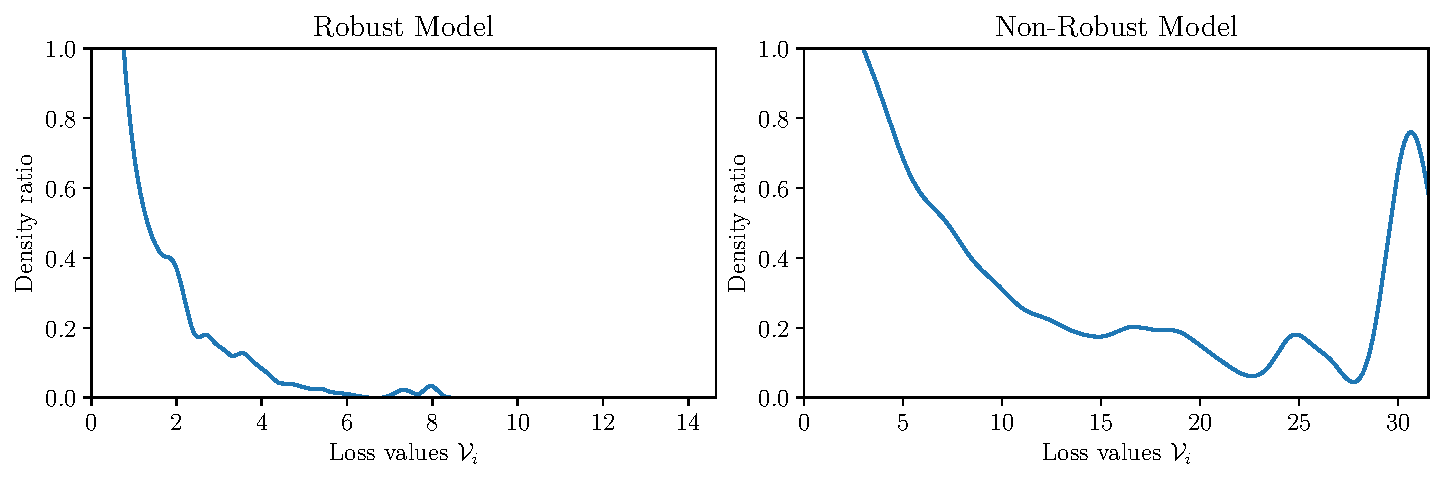
\includegraphics[width=\textwidth]{Figures/density_ratio.pdf}
    \caption{Distribution of the values for robust and non-robust models. We use a gaussian kernel density estimator to estimate the density.}
\label{fig:distrib_values}
\end{figure}

\section*{Societal Impact}
\label{broader_impact}
We introduce the online threat model which aims to capture a new domain for adversarial attack research against streaming data. Such a threat model exposes several new security and privacy risks. For example, using online algorithms, adversaries may now tailor their attack strategy to attacking a small subset of streamed data but still cause significant damage to downstream models e.g. the control system of an autonomous car. On the other hand our research also highlights the need and importance of stateful defence strategies that are capable of mitigating such online attacks. On the theoretical side the development and analysis of \algoname \ has many potential applications outside of adversarial attacks broadly categorized as resource allocation problems. As a concrete example one can consider advertising auctions which provide the main source of monetization for a variety of internet services including search engines, blogs, and social networking sites. Such a scenario is amenable to being modelled as a secretary problem as an advertiser may be able to estimate accurately the bid required to win a particular auction, but may not be privy to the trade off for future auctions.

